\documentclass{article}

\def\ParSkip{} 
% Packages
\usepackage{amssymb,amsmath,amsthm,bbm}
\usepackage{verbatim,float,url,dsfont}
\usepackage{graphicx,subfigure,psfrag}
\usepackage{algorithm,algorithmic}
\usepackage{mathtools,enumitem}
\usepackage{multirow}
\usepackage{ragged2e}
\usepackage{xr-hyper}
\usepackage{array}

\usepackage[colorlinks=true,citecolor=blue,urlcolor=blue,linkcolor=blue]{hyperref}
\usepackage[margin=1in]{geometry}
\usepackage[round]{natbib}

\usepackage[utf8]{inputenc} % allow utf-8 input
\usepackage[T1]{fontenc}    % use 8-bit T1 fonts
\usepackage{booktabs}       % professional-quality tables
\usepackage{nicefrac}         % compact symbols for 1/2, etc.
\usepackage{microtype}      % microtypography

\ifdefined\TimesFont 
\usepackage{times} % use times font
\fi

\ifdefined\ParSkip 
\usepackage{parskip} % use par skip
\fi

% Theorems and such
\newtheorem{theorem}{Theorem}
\newtheorem{lemma}{Lemma}
\newtheorem{corollary}{Corollary}
\newtheorem{proposition}{Proposition}
\theoremstyle{definition}
\newtheorem{remark}{Remark}
\newtheorem{definition}{Definition}

% Assumption
\newtheorem*{assumption*}{\assumptionnumber}
\providecommand{\assumptionnumber}{}
\makeatletter
\newenvironment{assumption}[2]{
  \renewcommand{\assumptionnumber}{Assumption #1#2}
  \begin{assumption*}
  \protected@edef\@currentlabel{#1#2}}
{\end{assumption*}}
\makeatother

% Widebar
\makeatletter
\newcommand*\rel@kern[1]{\kern#1\dimexpr\macc@kerna}
\newcommand*\widebar[1]{%
  \begingroup
  \def\mathaccent##1##2{%
    \rel@kern{0.8}%
    \overline{\rel@kern{-0.8}\macc@nucleus\rel@kern{0.2}}%
    \rel@kern{-0.2}%
  }%
  \macc@depth\@ne
  \let\math@bgroup\@empty \let\math@egroup\macc@set@skewchar
  \mathsurround\z@ \frozen@everymath{\mathgroup\macc@group\relax}%
  \macc@set@skewchar\relax
  \let\mathaccentV\macc@nested@a
  \macc@nested@a\relax111{#1}%
  \endgroup
}
\makeatother

% Min and max 
\DeclareMathOperator*{\argmin}{argmin}
\DeclareMathOperator*{\argmax}{argmax}
\DeclareMathOperator*{\minimize}{minimize}
\DeclareMathOperator*{\maximize}{maximize}
\DeclareMathOperator*{\find}{find}
\DeclareMathOperator{\st}{subject\,\,to}

% Other operators
\DeclareMathOperator{\Cov}{Cov}
\DeclareMathOperator{\Var}{Var}
\DeclareMathOperator{\dm}{dim}
\DeclareMathOperator{\col}{col}
\DeclareMathOperator{\row}{row}
\DeclareMathOperator{\nul}{null}
\DeclareMathOperator{\rank}{rank}
\DeclareMathOperator{\nuli}{nullity}
\DeclareMathOperator{\spa}{span}
\DeclareMathOperator{\sign}{sign}
\DeclareMathOperator{\supp}{supp}
\DeclareMathOperator{\diag}{diag}
\DeclareMathOperator{\aff}{aff}
\DeclareMathOperator{\conv}{conv}
\DeclareMathOperator{\dom}{dom}
\DeclareMathOperator{\tr}{tr}
\DeclareMathOperator{\df}{df}

% Other shortcuts 
\def\R{\mathbb{R}}
\def\C{\mathbb{C}}
\def\E{\mathbb{E}}
\def\P{\mathbb{P}}
\def\T{\mathsf{T}}
\def\half{\frac{1}{2}}
\def\df{\mathrm{df}}
\def\hy{\hat{y}}
\def\hf{\hat{f}}
\def\hmu{\hat{\mu}}
\def\halpha{\hat{\alpha}}
\def\hbeta{\hat{\beta}}
\def\htheta{\hat{\theta}}
\def\indep{\perp\!\!\!\perp}
\def\th{^{\textnormal{th}}}

\def\cA{\mathcal{A}}
\def\cB{\mathcal{B}}
\def\cD{\mathcal{D}}
\def\cE{\mathcal{E}}
\def\cF{\mathcal{F}}
\def\cG{\mathcal{G}}
\def\cK{\mathcal{K}}
\def\cH{\mathcal{H}}
\def\cI{\mathcal{I}}
\def\cL{\mathcal{L}}
\def\cM{\mathcal{M}}
\def\cN{\mathcal{N}}
\def\cP{\mathcal{P}}
\def\cS{\mathcal{S}}
\def\cT{\mathcal{T}}
\def\cW{\mathcal{W}}
\def\cX{\mathcal{X}}
\def\cY{\mathcal{Y}}
\def\cZ{\mathcal{Z}}


\title{Lecture 6: Autoregressive Integrated Moving Average Models \\ \smallskip  
\large Introduction to Time Series, Fall 2023 \\ \smallskip
Ryan Tibshirani}
\date{}

\begin{document}
\maketitle
\RaggedRight
\vspace{-50pt}

Related reading: Chapters 3.1, 3.3, and 3.6 in Shumway and Stoffer (SS);
Chapters 9.1--9.5 and 9.8--9.9 of Hyndman and Athanasopoulos (HA).   

\section{AR models}

\begin{itemize}
\item The \emph{autoregressive} (AR) model is one of the foundational legs of
  ARIMA models, which we'll cover bit by bit in this lecture. (Recall, you've
  already learned about AR models, which were introduced all the way back in our 
  first lecture)  

\item Precisely, an AR model of order $p \geq 0$, denoted AR($p$), is of the
  form 
  \begin{equation}
  \label{eq:ar_p}
  x_t = \sum_{j=1}^p \phi_j x_{t-j} + w_t
  \end{equation}
  where $w_t$, $t = 0, \pm 1, \pm 2, \pm 3, \dots$ is a white noise
  sequence. Note that we allow the time index to be negative here (we extend
  time back to $-\infty$), which will useful in what follows 

\item The coefficients $\phi_1,\dots,\phi_p$ in \eqref{eq:ar_p} are fixed
  (nonrandom), and we assume $\phi_p \not= 0$ (otherwise the order here would
  effectively be less than $p$). Note that in \eqref{eq:ar_p}, we have $\E(x_t)
  = 0$ for all $t$

\item If we wanted to allow for a nonzero but constant mean, then we could add
  an intercept to the model in \eqref{eq:ar_p}. We'll omit this for simplicity
  in this lecture  

\item A useful tool for expressing and working with AR models is the
  \emph{backshift operator}: this is an operator we denote by $B$ that takes a 
  given time series and shifts it back in time by one index,
  \[
  B x_t = x_{t-1}
  \]

\item We can extend this to powers, as in $B^2 x_t = B B x_t = x_{t-2}$, and so
  on, thus   
  \[
  B^k x_t = x_{t-k} 
  \]

\item Returning to \eqref{eq:ar_p}, note now that we can rewrite this as 
  \[
  x_t - \phi_1 x_{t-1} - \phi_2 - x_{t-2} - \cdots - \phi_p x_{t-p} = w_t  
  \]
  or in other words, using backshift notation 
  \begin{equation}
  \label{eq:ar_p_backshift}
  \Big(1 - \phi_1 B - \phi_2 B^2 - \cdots - \phi_p B^p \Big) x_t = w_t 
  \end{equation}

\item Hence \eqref{eq:ar_p_backshift} is just a compact way to represent the
  AR($p$) model \eqref{eq:ar_p} using the backshift operator $B$. Often, authors
  will write this model even more compactly as  
  \begin{equation}
  \label{eq:ar_p_operator}
  \phi(B) x_t = w_t 
  \end{equation}
  where $\phi(B) = 1 - \phi_1 B - \phi_2 B^2 - \cdots - \phi_p B^p$ is called
  the \emph{autoregressive operator} of order $p$, associated with the
  coefficients $\phi_1,\dots,\phi_p$

\item Figure \ref{fig:ar} shows two simple examples of AR processes
\end{itemize}

\begin{figure}[htb]
\centering
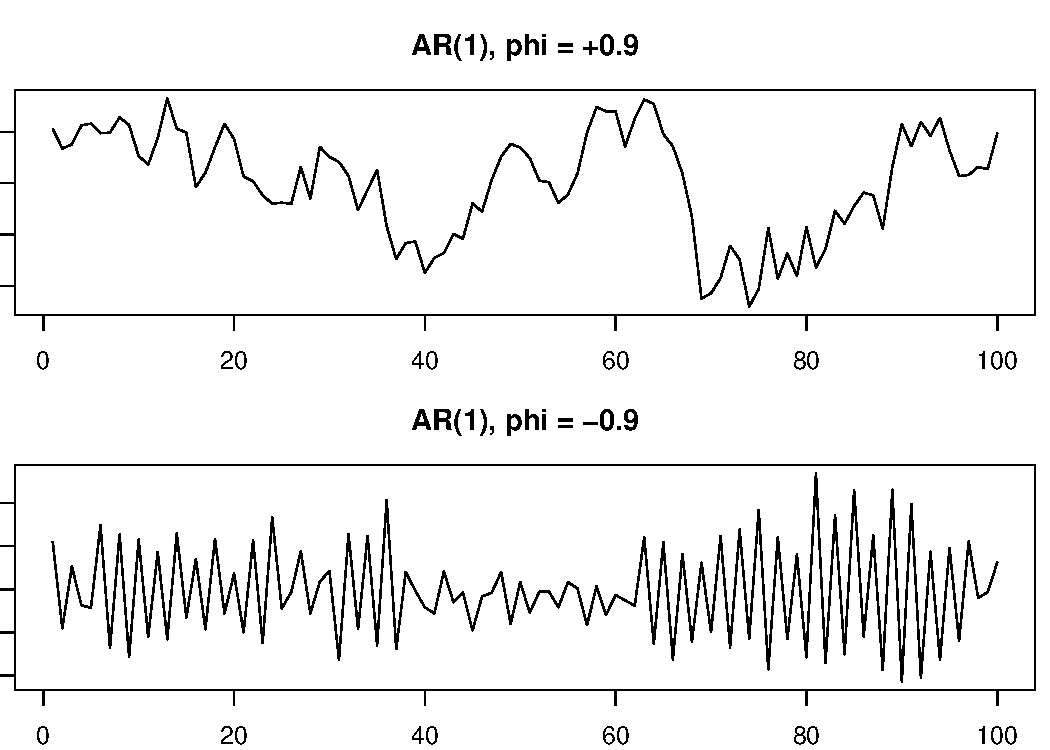
\includegraphics[width=0.85\textwidth]{fig/ar-1.pdf}
\caption{Two examples of AR(1) processes, with $\phi = \pm 0.9$.}
\label{fig:ar}
\end{figure}

\subsection{AR(1): auto-covariance and stationarity}

\begin{itemize}
\item A key question for us will be: \emph{under what conditions does the AR
    model  in \eqref{eq:ar_p}, or equivalently \eqref{eq:ar_p_operator}, define
    a stationary process?} 

\item The answer will turn out to be fairly sophisticated, but we can glean some
  intuition by starting with the AR(1) case: 
  \begin{equation}
  \label{eq:ar_1}
  x_t = \phi x_{t-1} + w_t 
  \end{equation}

\item Note that a random walk is the special case with $\phi = 1$. We already
  know (from previous lectures) that this is nonstationary, so certainly
  \eqref{eq:ar_1} cannot be stationary for any $\phi$

\item Unraveling the iterations, we get
  \begin{align*}
  x_t &= \phi^2 x_{t-2} + \phi w_{t-1} + w_t \\
  &= \phi^3 x_{t-3} + \phi^2 w_{t-2} + \phi w_{t-1} + w_t \\  
  &\vdots \\ 
  &= \phi^k x_{t-k} + \sum_{j=0}^k \phi^j w_{t-j} 
  \end{align*}

\item If $|\phi| < 1$, then we can send $k \to \infty$ in the last display to 
  get 
  \begin{equation}
  \label{eq:ar_1_stationary}
  x_t = \sum_{j=0}^\infty \phi^j w_{t-j} 
  \end{equation}
  This is called the \emph{stationary representation} of the AR(1) process
  \eqref{eq:ar_1} 

\item Why is it called this? We can compute the auto-covariance function,
  writing $\sigma^2 = \Var(w_t)$ for the noise variance, as
  \begin{align}
  \nonumber
  \Cov(x_t, x_{t+h}) &= \Cov\bigg( \sum_{j=0}^\infty \phi^j w_{t-j}, 
  \sum_{\ell=0}^\infty \phi^\ell w_{t+h-\ell} \bigg) \\
  \nonumber
  &= \sum_{j,\ell=0}^\infty \phi^j \phi^\ell \Cov( w_{t-j}, w_{t+h-\ell} ) \\ 
  \nonumber
  &= \sum_{j=0}^\infty \phi^j \phi^{j+h} \sigma^2 \\
  \nonumber
  &= \sigma^2 \phi^h \sum_{j=0}^\infty \phi^{2j} \\
  \label{eq:ar_1_auto_cov}
  &= \sigma^2 \frac{\phi^h}{1 - \phi^2}    
  \end{align}
  where we used the fact that \smash{$\sum_{j=0}^\infty b^j = 1/(1-b)$} for $|b|
  < 1$. Since the auto-covariance in the last line only depends on $h$, we can
  see that the AR(1) process is indeed stationary

\item To reiterate, the representation \eqref{eq:ar_1_stationary}, and the
  auto-covariance calculation just given, would have not been possible unless
  $|\phi| < 1$. This condition is required in order for the AR(1) process to
  have a stationary representation. We will see later that we can generalize
  this to a condition that applies to an AR($p$), yielding an analogous
  conclusion. The conclusion we will be looking for is explained next  
\end{itemize}

\subsection{Causality (no, not the usual kind)}

\begin{itemize}
\item Now we will introduce a concept called \emph{causality}, which generalizes
  what we just saw falls out of an AR(1) when $|\phi| < 1$. This is a slightly
  unfortunate bit of nomenclature that nonetheless seems to be common in the
  time series literature. It has really nothing to do with causality used in the
  broader sense in statistics. We will ... somewhat begrudgingly ... stick with
  the standard nomenclature in time series here  

\item We say that a series $x_t$, $t = 0, \pm 1, \pm 2, \pm 3, \dots$ is
  \emph{causal} provided that it can be written in the form
  \begin{equation}
  \label{eq:causal}
  x_t = \sum_{j=0}^\infty \psi_j w_{t-j}
  \end{equation}
  for a white noise sequence $w_t$, $t = 0, \pm 1, \pm 2, \pm 3, \dots$, and
  coefficients such that \smash{$\sum_{j=0}^\infty |\psi_j| < \infty$}  

\item You should think of this as a generalization of
  \eqref{eq:ar_1_stationary}, where we allow for arbitrary coefficients
  $\psi_0,\psi_1,\psi_2,\dots$, subject to an absolute summability condition  

\item It is straightforward to check that causality actually implies
  stationarity: we can just compute the auto-covariance function in
  \eqref{eq:causal}, similar to the above calculation:
    \begin{align*}
  \Cov(x_t, x_{t+h}) &= \Cov\bigg( \sum_{j=0}^\infty \psi_j w_{t-j}, 
  \sum_{\ell=0}^\infty \psi_\ell w_{t+h-\ell} \bigg) \\
  &= \sum_{j,\ell=0}^\infty \psi_j \psi_\ell \Cov( w_{t-j}, w_{t+h-\ell} ) \\
  &= \sigma^2 \sum_{j=0}^\infty \psi_j \psi_{j+h}
  \end{align*}
  The summability condition ensures that these calculations are well-defined and
  that the last display is finite. Since this only depends on $h$, we can see
  that the process is indeed stationary

\item Thus, to emphasize, causality actually tells us \emph{more} than
  stationary: it is stationary ``plus'' a representation a linear filter of past
  white noise variates, with summable coefficients

\item Note that when $\psi_j = \phi^j$, the summability condition
  \smash{$\sum_{j=0}^\infty |\psi_j| < \infty$} is true if and only if $|\phi| <
  1$. Hence what we actually proved above for AR(1) was that it is causal if and
  only if $|\phi| < 1$. And it is this condition---for causality---that we will
  actually generalize for AR($p$) models, and beyond 
\end{itemize}

\section{MA models}

\begin{itemize}
\item A \emph{moving average} (MA) model is ``dual'', in a colloquial sense, to
  the AR model. Instead of having $x_t$ evolve according to a linear combination
  of the recent past, the \emph{errors} in the model evolve according to a
  linear combination of white noise

\item Precisely, an MA model of order $q \geq 0$, denoted MA($q$), is of the
  form 
  \begin{equation}
  \label{eq:ma_q}
  x_t = w_t + \sum_{j=1}^q \theta_j w_{t-j} 
  \end{equation}
  where $w_t$, $t = 0, \pm 1, \pm 2, \pm 3, \dots$ is a white noise
  sequence

\item The coefficients $\theta_1,\dots,\theta_q$ in \eqref{eq:ma_q} are fixed
  (nonrandom), and we assume $\theta_q \not= 0$ (otherwise the order here would 
  effectively be less than $q$). Note that in \eqref{eq:ma_q}, we have $\E(x_t)
  = 0$ for all $t$ 

\item Again, we can rewrite \eqref{eq:ma_q}, using backshift notation, as 
  \begin{equation}
  \label{eq:ma_q_backshift}
  x_t = \Big(1 + \theta_1 B + \theta_2 B^2 + \cdots + \theta_q B^q \Big) w_t   
  \end{equation}

\item Often, authors will write \eqref{eq:ma_q_backshift} even more compactly as   
  \begin{equation}
  \label{eq:ma_q_operator}
  x_t = \theta(B) w_t 
  \end{equation}
  where $\theta(B) = 1 + \theta_1 B + \theta_2 B^2 + \cdots + \theta_q B^q$ is
  called the \emph{moving average operator} of order $q$, associated with the
  coefficients $\theta_1,\dots,\theta_q$

\item Figure \ref{fig:ma} shows two simple examples of MA processes

\begin{figure}[htb]
\centering
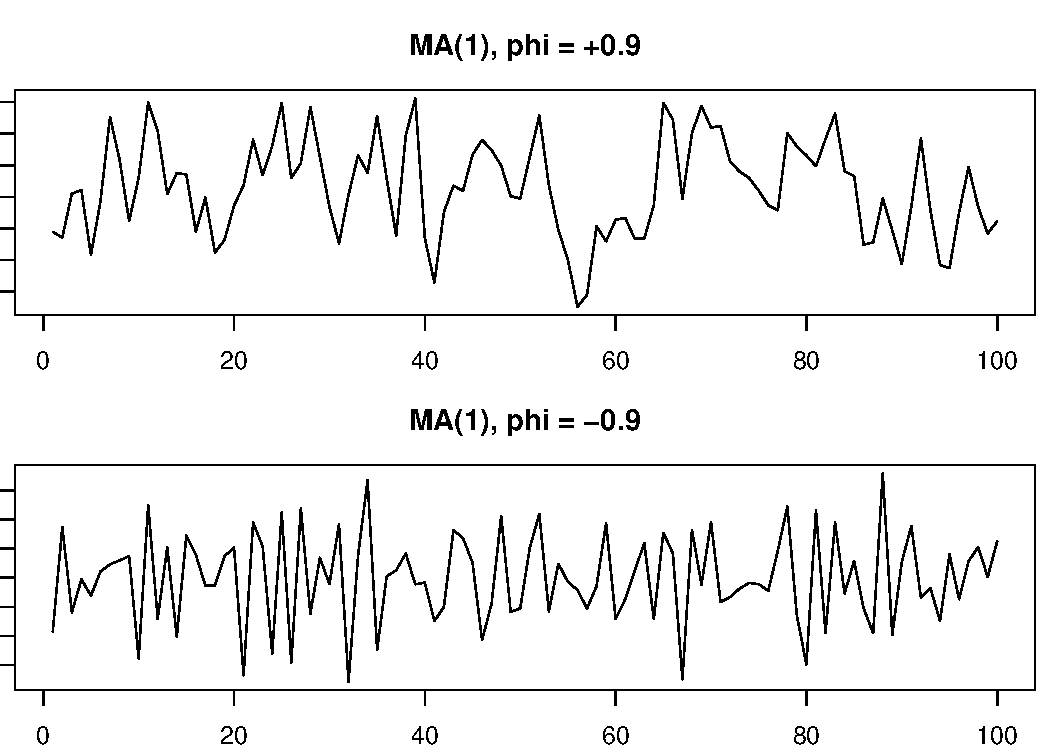
\includegraphics[width=0.85\textwidth]{fig/ma-1.pdf}
\caption{Two examples of MA(1) processes, with $\theta = \pm 0.9$.}
\label{fig:ma}
\end{figure}
\end{itemize}

\subsection{Stationarity}

\begin{itemize}
\item Unlike AR processes, an MA process \eqref{eq:ma_q} is stationary \emph{for
    any values of the parameters $\theta_1,\dots,\theta_q$}

\item To check this, we compute the auto-covariance function using a similar
  calculation to those we've done before, writing $\theta_0 = 1$ for
  convenience,
  \begin{align}
  \nonumber
  \Cov(x_t, x_{t+h}) &= \Cov\bigg( \sum_{j=0}^q \theta_j w_{t-j}, 
  \sum_{\ell=0}^q \theta_\ell w_{t+h-\ell} \bigg) \\
  \nonumber
  &= \sum_{j,\ell=0}^q \theta_j \theta_\ell \Cov( w_{t-j}, w_{t+h-\ell} ) \\
  \label{eq:ma_q_auto_cov}
  &= \sum_{j \,:\, 0 \leq j,  j +h \leq q} \theta_j \theta_{j+h} \sigma^2
  \end{align}
  Since this only depends on $h$, we can see that the process is indeed
  stationary 

\item The similarity in these calculations brings us to pause to emphasize the
  following connection: \emph{an AR(1) model with $|\phi| < 1$ is also a
    particular infinite-order MA model}, as we saw in the stationary
  representation \eqref{eq:ar_1_stationary}. We will see later that there are
  more general connections to be made
\end{itemize}

\subsection{MA(1): issues with non-uniqueness}

\begin{itemize}
\item Consider the MA(1) model:
  \begin{equation}
  \label{eq:ma_1}
  x_t = w_t + \theta w_{t-1}
  \end{equation}

\item According to \eqref{eq:ma_q_auto_cov}, we can compute its auto-covariance 
  simply (recalling $\theta_0 = 1$) as
  \begin{equation}
  \label{eq:ma_1_auto_cov}  
  \gamma_x(h) = \begin{cases}
  (1+\theta^2) \sigma^2 & h = 0 \\
  \theta \sigma^2 & |h| = 1 \\
  0 & |h| > 1 \\
  \end{cases}
  \end{equation}

\item The corresponding auto-correlation function is thus
  \[
  \rho(h) = \begin{cases}
  1 & h = 0 \\
  \frac{\theta}{1+\theta^2} & |h| = 1 \\ 
  0 & |h| > 1 \\
  \end{cases}
  \]

\item If we look carefully, then we can see a problem lurking here: the
  auto-correlation function is unchanged if we replace $\theta$ by $1/\theta$

\item And in fact, the auto-covariance function \eqref{eq:ma_1_auto_cov} is
  unchanged if we replace $\theta$ and $\sigma^2$ with $1/\theta$ and $\sigma^2
  \theta^2$; e.g., try $\theta = 5$ and $\sigma^2 = 1$, and $\theta = 1/5$ and
  $\sigma^2 = 25$, you'll find that the auto-covariance function is the same in
  both cases 

\item This is not good because it means we cannot detect the difference in an
  MA(1) model with parameter $\theta$ and normal noise with variance $\sigma^2$ 
  from another MA(1) model with parameter $1/\theta$ and normal noise with
  variance $\sigma^2 \theta^2$

\item In other words, there is some \emph{non-uniqueness} of \emph{redundancy}
  in the parametrization---different choices of parameters will actually lead to
  the same behavior in the model at the end

\item In the MA(1) case, the convention is to simply choose the parametrization
  with $|\theta| <  1$. Note that we can write
  \[
  w_t = -\theta w_{t-1} + x_t 
  \]
  which is like an AR(1) process with the roles of $x_t$ and $w_t$
  reversed. Thus by the same arguments that led to \eqref{eq:ar_1_stationary},
  when $|\theta| < 1$, we now have 
  \begin{equation}
  \label{eq:ma_1_invertible}
  w_t = \sum_{j=0}^\infty (-\theta)^j x_{t-j} 
  \end{equation}
  This is called the \emph{invertible representation} of the MA(1) process
  \eqref{eq:ma_1} 

\item We will see soon that we can generalize this to a condition that applies
  to a general MA($q$), yielding an analogous conclusion. The conclusion we will
  be looking for is explained next 
\end{itemize}

\subsection{Invertibility}

\begin{itemize}
\item Before we turn to ARMA models, we define one last concept called
  \emph{invertibility}, which generalizes what we just saw for MA(1) when
  $|\theta| < 1$ 

\item We say that a series $x_t$, $t = 0, \pm 1, \pm 2, \pm 3, \dots$ is
  \emph{invertible} provided that it can be written in the form
  \begin{equation}
  \label{eq:invertible}
  w_t = \sum_{j=0}^\infty \pi_j x_{t-j}
  \end{equation}
  for a white noise sequence $w_t$, $t = 0, \pm 1, \pm 2, \pm 3, \dots$,
  and coefficients such that \smash{$\sum_{j=0}^\infty |\pi_j| < \infty$}, where 
  we set $\pi_0 = 1$

\item You should think of this as a generalization of
  \eqref{eq:ma_1_invertible}, where we allow for arbitrary coefficients
  $\pi_1,\pi_2,\dots$, subject to an absolute summability condition   

\item And of course, note how invertibility \eqref{eq:invertible} is kind of an
  opposite condition to causality \eqref{eq:causal}  
\end{itemize}

\section{ARMA models}

\begin{itemize}
\item AR and MA models have complementary characteristics. The auto-covariance
  of an AR model generally decays away from $h=0$, whereas that for an MA
  process has finite support---in other words, at a certain lag, variates along
  an MA sequence are completely uncorrelated. You can compare
  \eqref{eq:ar_1_auto_cov} and \eqref{eq:ma_1_auto_cov} for the AR(1) and MA(1)
  models

\item (The spectral perspective, by the way, provides another nice way of
  viewing these complementary characteristics. In the spectral domain, the story
  is somewhat flipped: the spectral density of an MA process generally decays
  away from $\omega=0$, whereas that for an AR process can be much more locally
  concentrated around particular frequencies; recall our examples from the last
  lecture) 

\item Sure, there is some duplicity in representation here, as we will see---we
  can write some AR models as infinite-order MA models, and some MA models as  
  infinite-order AR models. But that's OK! We can take the most salient features
  that each model represents, and combine them to get a simple model formulation
  that exhibits both sets of features, simultaneously. This is exactly what an
  ARMA model does       

\item Precisely, an ARMA model of orders $p,q \geq 0$, denoted ARMA($p,q$), is
  of the form 
  \begin{equation}
  \label{eq:arma_pq}
  x_t = \sum_{j=1}^p \phi_j x_{t-j} + \sum_{j=0}^q \theta_j w_{t-j}  
  \end{equation}
  where $w_t$, $t = 0, \pm 1, \pm 2, \pm 3, \dots$ is a white noise sequence 

\item The coefficients $\phi_1,\dots,\phi_p,\theta_0,\dots,\theta_q$ in
  \eqref{eq:arma_pq} are fixed (nonrandom), and we assume $\phi_p,\theta_q \not=
  0$, and we set $\theta_0 = 1$. Note that in \eqref{eq:arma_pq}, we have
  $\E(x_t) = 0$ for all $t$ 

\item As before, we can represent an ARMA model more compactly using backshift 
  notation, rewriting \eqref{eq:arma_pq} as
  \begin{equation}
  \label{eq:arma_pq_backshift}
  \Big(1 - \phi_1 B - \phi_2 B^2 - \cdots - \phi_p B^p \Big) x_t = 
  \Big(1 + \theta_1 B + \theta_2 B^2 + \cdots + \theta_q B^q \Big) w_t   
  \end{equation}

\item Often, authors will write \eqref{eq:arma_pq_backshift} even more compactly
  as    
  \begin{equation}
  \label{eq:arma_pq_operator}
  \phi(B) x_t = \theta(B) w_t  
  \end{equation}
  where $\phi(B) = 1 - \phi_1 B - \phi_2 B^2 - \cdots - \phi_p B^p$ and
  $\theta(B) = 1 + \theta_1 B + \theta_2 B^2 + \cdots + \theta_q B^q$ are the AR 
  and MA operators, as before 
\end{itemize}

\subsection{Parameter redundancy}

\begin{itemize}
\item For ARMA models, there is an issue of parameter redundancy, just like
  there are for MA models. If $\eta(B)$ is any (invertible) operator, then we
  can transform \eqref{eq:arma_pq_operator} by applying $\eta(B)$ on both sides,  
  \[
  \eta(B) \phi(B) x_t = \eta(B) \theta(B) w_t  
  \]
  which may look like a different model, but the dynamics are entirely the
  same  

\item As an example, consider white noise $x_t = w_t$, and multiply both sides
  by $\eta(B) = 1 - B/2$. This gives:
  \[
  x_t = \frac{1}{2} x_{t-1} + w_t - \frac{1}{2} w_{t-1}
  \]
  which looks like an ARMA(1,1) model, but it is nothing else that white noise!
 
\item How do we resolve this issue? Doing so requires introducing another
  concept. The \emph{AR and MA polynomials} associated with the ARMA process
  \eqref{eq:arma_pq} are 
  \begin{align}
  \label{eq:ar_p_polynomial}
  \phi(z) &= 1 - \phi_1 z - \phi_2 z^2 - \cdots - \phi_p z^p \\
  \label{eq:ma_q_polynomial}
  \theta(z) &= 1 + \theta_1 z + \theta_2 z^2 + \cdots + \theta_q z^q
  \end{align}
  respectively. To be clear, these are polynomials over \emph{complex numbers}
  $z \in \C$. (Note that these are just what we get by taking the AR and MA
  operators, and replacing the backshift operator $B$ by a complex argument $z$) 

\item As it turns out, several important properties of ARMA models can be 
  derived by placing conditions on the AR and MA polynomials. Here we'll see the
  first one, to deal with parameter redundancy: \emph{when we speak of an ARMA
    model, we implicitly assume that the AR and MA polynomials $\phi(z)$ and
    $\theta(z)$, in \eqref{eq:ar_p_polynomial} and \eqref{eq:ma_q_polynomial},
    have no common factors}. This rules out a case like   
  \[
  x_t = \frac{1}{2} x_{t-1} + w_t - \frac{1}{2} w_{t-1}
  \]
  because the polynomials each have $1-z/2$ as a common factor. Hence we do not  
  even refer to the above as an ARMA(1,1) model
\end{itemize}

\subsection{Causality and invertibility}

\begin{itemize}
\item Now we learn about two more conditions on the AR and MA polynomials that
  imply important general properties of the underlying ARMA process, and
  generalize calculations we saw earlier for AR(1) and MA(1) models

\item Before we describe these, we recall the following terminology: for a
  polynomial \smash{$P(z) = \sum_{j=0}^k a_j z^j$}, we say that $z$ is a
  \emph{root} of $P$ provided $P(z) = 0$

\item And we say that a point $z \in \C$ lies \emph{outside of the unit circle} 
  (in the complex plane $\C$) provided that $|z| > 1$, where $|z|$ is the
  complex modulus of $z$ (recall $|z|^2 = \mathrm{Re}\{z\}^2 +
  \mathrm{Im}\{z\}^2$)     

\item The first property: \emph{the ARMA process \eqref{eq:arma_pq} has a causal
    representation \eqref{eq:causal} if and only if all roots of the AR
    polynomial \eqref{eq:ar_p_polynomial} lie outside of the unit circle}. The
  coefficients $\psi_0,\psi_1,\psi_2,\dots$ in the causal representation can be
  determined by solving  
  \[
  \psi(z) = \phi(z)^{-1} \theta(z) \iff 
  \sum_{j=0}^\infty \psi_j z^j = \frac{1 + \theta_1 z + \theta_2 z^2 + \cdots +
    \theta_q z^q}{1 - \phi_1 z - \phi_2 z^2 - \cdots - \phi_p z^p}, \quad
  \text{for $|z| < 1$}
  \]

\item The second property: \emph{the ARMA process \eqref{eq:arma_pq} is
    invertible \eqref{eq:invertible} if and only if all roots of the MA
    polynomial \eqref{eq:ma_q_polynomial} lie outside of the unit circle}. The  
  coefficients $\pi_1,\pi_2,\dots$ in the invertible representation can be 
  determined by solving   
  \[
  \pi(z) = \theta(z)^{-1} \phi(z) \iff 
  \sum_{j=0}^\infty \pi_j z^j = \frac{1 - \phi_1 z - \phi_2 z^2 - \cdots -
    \phi_p z^p}{1 + \theta_1 z + \theta_2 z^2 + \cdots + \theta_q z^q}, \quad 
  \text{for $|z| < 1$}
  \]

\item (As an aside, you can see that parameter redundancy issues would not
  affect the causal and invertible representations, as they shouldn't, because
  any common factors in $\phi(z)$ and $\theta(z)$ would cancel in their ratios 
  which determine the coefficients in the causal and invertible expansions)  

\item Interestingly, these results can also be interpreted as follows:
  \begin{itemize}
  \item An AR($q$) process, such that the roots of $\phi$ lie outside the unit
    circle, can also be written as an MA($\infty$) process (this is what
    causality \eqref{eq:causal} means)

  \item An MA($q$) process, such that the roots of $\theta$ lie outside the 
  unit circle, can also be written as an AR($\infty$) process (this is what 
  invertibility \eqref{eq:invertible} means, as it says
  \smash{$x_t = -\sum_{j=1}^\infty \pi_j x_{t-j} + w_t$})
  \end{itemize}

\item We won't cover the proofs of these properties or go into further details
  about them. But you will see several hints of their significance (what the
  causal and invertible representations allow us to do) in what follows. At 
  a high-level, they are worth knowing because they are considered foundational 
  results for ARMA modeling (just like it is worth knowing foundations for 
  regression modeling, and so on). You can refer to Appendix B.2 of SS for
  proofs, or read more in Chapter 3 of SS

\item Also, recall that causality implies stationarity, so what we have just
  learned is the general result that renders an ARMA($p,q$) process stationary 

\item Finally, as a summary, here are three equivalent ways to represent a
  causal, invertible ARMA($p,q$) model:
  \begin{align*}
  &\phi(B) x_t = \theta(B) w_t \\
  &x_t = \psi(B) w_t, \quad \text{for $\psi(B) = \phi(B)^{-1} \theta(B)$} \\ 
  &\pi(B) x_t = w_t, \quad \text{for $\pi(B) = \theta(B)^{-1} \phi(B)$} 
  \end{align*}
\end{itemize}

\subsection{Auto-covariance}

\begin{itemize}
\item The auto-covariance for an MA($q$) model was already given in
  \eqref{eq:ma_q_auto_cov}. We can see that it is zero when $|h| > q$: this is a
  signature structure of the MA($q$) model 

\item The auto-covariance for a causal AR(1) model was given in
  \eqref{eq:ar_1_auto_cov}. We can see that it decays away from $h=0$: this is 
  a signature structure of AR models. But what does the precise auto-covariance
  look like for a general causal AR($p$) model? How about a general causal
  ARMA($p,q$) model?  

\item The answer is much more complicated, but still possible to characterize
  precisely. We'll do it first for an AR($p$) model, and then look at an
  ARMA($p,q$) model, which will have an analogous behavior 

\item For an AR($p$) model \eqref{eq:ar_p}, assumed causal (i.e., all roots of
  $\phi(z)$ are outside of the unit circle), we can focus on the auto-covariance  
  at lags $ h \geq 0$ (without a loss of generality, because $\gamma_x$ is
  symmetric around zero), 
  \[
  \Cov(x_t, x_{t+h}) = \sum_{j=1}^p \phi_j \Cov(x_t, x_{t+h-j}) + \Cov(x_t,
  w_{t+h})  
  \]

\item The last term on the right-hand side zero for $h>0$; recall, $x_t$ is a  
  causal process, and only depends on white noise in the past. On the other
  hand, when $h=0$, writing \smash{$x_t = \sum_{j=0}^\infty \psi_j
    w_{t-j}$}, 
  \[
  \Cov(x_t, w_t) = \sum_{j=0}^\infty \psi_j \Cov(w_{t-j}, w_t) =  \sigma^2
  \psi_0   
  \]

\item Combining the last two displays, we learn that the auto-covariance
  function satisfies 
  \begin{align*}
  &\gamma_x(h) - \sum_{j=1}^p \phi_j \gamma_x(h-j) = 0, \quad h > 0 \\ 
  &\gamma_x(0) - \sum_{j=1}^p \phi_j \gamma_x(-j) = \sigma^2 \psi_0, 
  \end{align*}

\item This is called a \emph{difference equation} of order $p$ for the
  auto-covariance function $\gamma_x$. Some simple difference equations can be
  solved explicitly without complicated mathematics, but to solve a difference  
  equation in general requires knowing something (again) about the roots of a
  certain complex polynomial associated with the difference equation, when it is
  represented in operator notation. You can read Chapter 3.2 of SS for an
  introduction to the theory of difference equations

\item For an AR($p$) model, it turns out we can solve the difference equation in
  the 
  last display and get
  \begin{equation}
  \label{eq:ar_p_auto_cov}
  \gamma_x(h) = P_1(h) z_1^{-h} + \cdots + P_r(h) z_r^{-h}
  \end{equation}
  where each $P_j$ is a polynomial, and each $z_j$ is a root of the AR
  polynomial $\phi$. Because each $|z_j| > 1$ (all roots lie outside the unit
  circle), we see that the auto-covariance function will decay to zero as $h \to
  \infty$. In the case that some roots are complex, then what will actually 
  happen is that the auto-covariance will dampen to zero but in doing so
  oscillate in a sinusoidal fashion

\item Now what about an ARMA($p,q$) model \eqref{eq:arma_pq}, assumed
  causal? Similarly, we can focus on the auto-covariance a lags $h \geq 0$, 
  \[
  \Cov(x_t, x_{t+h}) = \sum_{j=1}^p \phi_j \Cov(x_t, x_{t+h-j}) + \sum_{j=0}^q 
  \theta_j \Cov(x_t, w_{t+h-j})  
  \]

\item The last term on the right-hand side zero for $h>q$, whereas when $h \leq
  q$, writing \smash{$x_t = \sum_{\ell=0}^\infty \psi_\ell  w_{t-\ell}$}, we see
  that for $j \geq h$, 
  \[
  \Cov(x_t, w_{t+h-j}) = \sum_{\ell=0}^\infty \psi_\ell \Cov(w_{t-\ell},
  w_{t+h-j}) = \sigma^2 \psi_{j-h}   
  \]

\item Combining the last two displays, we learn that the auto-covariance
  function satisfies 
  \begin{alignat*}{2}
  &\gamma_x(h) - \sum_{j=1}^p \phi_j \gamma_x(h-j) = 0, \quad &&h > q \\ 
  &\gamma_x(h) - \sum_{j=1}^p \phi_j \gamma_x(h-j) = \sigma^2 \sum_{j=h}^q
    \psi_{j-h}, \quad &&h \leq q
  \end{alignat*}

\item This is again a difference equation of order $p$ that determines
  $\gamma_x$, but the boundary condition (what happens when $h \leq q$) is more
  complicated. Nonetheless, the solution is still the form
  \eqref{eq:ar_p_auto_cov}, and the qualitative behavior is still the same as in 
  the AR($p$) case   

\item Figure \ref{fig:auto_cor}, top row, shows sample auto-correlation
  functions for simple MA and AR models 

\begin{figure}[htb]
\centering
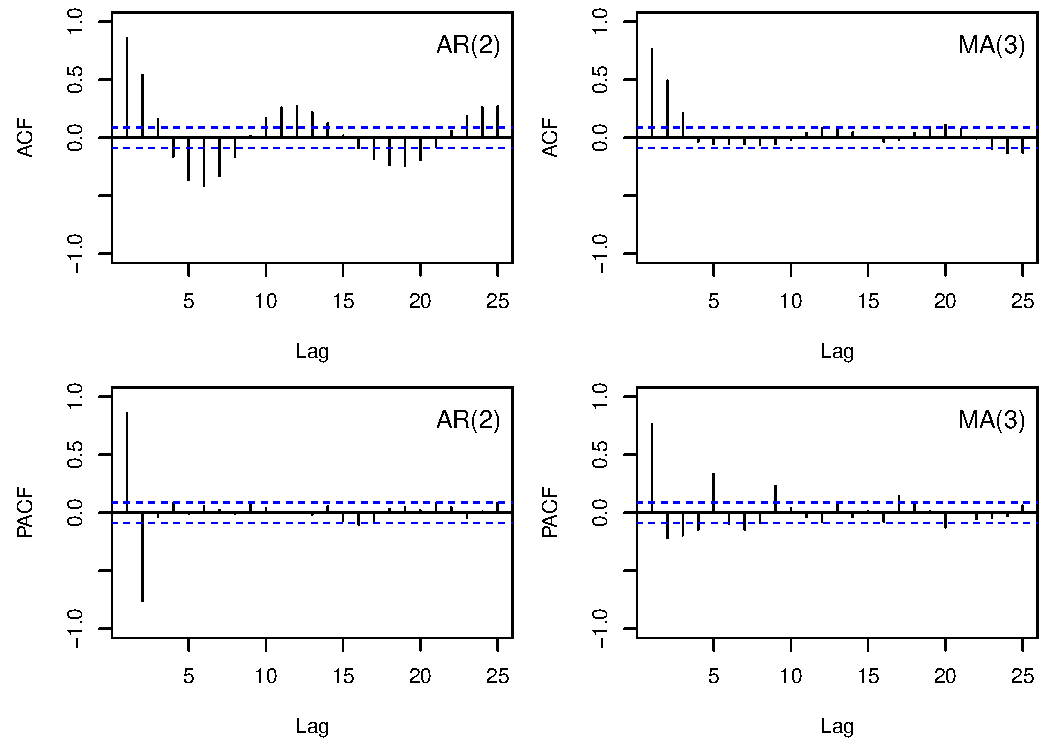
\includegraphics[width=0.85\textwidth]{fig/auto-cor-1.pdf}
\caption{Top row: sample auto-correlation functions for data from AR(2) and
  MA(3) models. Bottom row: sample partial auto-correlation functions for these
  same data.} 
\label{fig:auto_cor}
\end{figure}
\end{itemize}

\subsection{Partial auto-covariance}

\begin{itemize}
\item The auto-covariance function for an MA model provides a considerable
  amount of information that will help identify its structure: since it is zero
  for lags $h>q$, if we were to compute a sample version based on data, then by
  seeing where the sample auto-correlation ``cuts off'', we could roughly
  identify the order $q$ of the underlying MA process (see top right of Figure 
  \ref{fig:auto_cor} again)   

\item For an AR (or ARMA) model, this is not the case. As we saw from
  \eqref{eq:ar_p_auto_cov}, the auto-covariance decays to zero, but this tells
  us little about the AR order of dependence $p$ (see also top left of Figure 
  \ref{fig:auto_cor}). Thus it is worth pursuing a type of \emph{modified}
  correlation function for the AR model that behaves like the auto-correlation
  does for the MA model 

\item Such a modification will be given to us by the \emph{partial
    auto-correlation function}. In general, the partial correlation between
  random variables $X,Y$ given $Z$ is denoted \smash{$\rho_{XY|Z}$} and defined
  as    
  \begin{align*}
  &\rho_{XY|Y} = \Cor(X - \hat{X}, Y - \hat{Y}), \quad \text{where} \\
  &\text{$\hat{X}$ is the linear regression of $X$ on $Z$}, \quad \text{and} \\
  &\text{$\hat{Y}$ is the linear regression of $Y$ on $Z$}
  \end{align*}
  Here, and in what follows, by ``linear regression'' we mean regression in the
  population sense, so that precisely \smash{$\hat{X} = Z^\T \Cov(Z)^{-1}
    \E(ZX)$} and \smash{$\hat{Y} = Z^\T \Cov(Z)^{-1} \E(ZY)$}   

\item Said differently, the partial correlation of two random variables given
  $Z$ is the correlation \emph{after we remove (``partial out'') the linear
    dependence of each random variable on $Z$}     

\item We note that when $X,Y,Z$ are jointly normal, then this definition
  coincides with conditional correlation: \smash{$\rho_{XY|Z} = \Cor(X,Y|Z)$},
  but not in general 

\item We are now ready to define the partial auto-correlation function for a
  stationary time series $x_t$, $t = 0, \pm 1, \pm 2, \pm 3, \dots$, denoted
  $\phi_x(h)$ at a lag $h$. Without a loss of generality we will only define it
  for $h \geq 0$, since it will be symmetric around zero (due to stationarity). 
  First, at lag $h=0$ or $h=1$, we simply define: 
  \begin{align*}
  \phi_x(0) &= 1 \\
  \phi_x(1) &= \Cor(x_t, x_{t+1}) 
  \end{align*}
  Next, at all lags $h \geq 2$, we define: 
  \begin{align*}
  &\phi_x(h) = \Cor(x_t - \hat{x}_t, x_{t+h} - \hat{x}_{t+h}), \quad
    \text{where} \\ 
  &\text{$\hat{x}_t$ is the linear regression of $x_t$ on
    $x_{t+1},\dots,x_{t+h-1}$}, \quad \text{and} \\ 
  &\text{$\hat{x}_{t+h}$ is the linear regression of $x_{t+h}$ on 
    $x_{t+1},\dots,x_{t+h-1}$}  
  \end{align*}

\item To best see the effect of this definition we can go straight back to the
  causal AR($p$) model. When $h>p$, it can be shown that the population linear 
  regression \smash{$\hat{x}_{t+h}$}, of $x_{t+h}$ on $x_{t+1},\dots,x_{t+h-1}$, 
  is 
  \[
  \hat{x}_{t+h} = \sum_{j=1}^p \phi_j x_{t+h-j}
  \]
  Thus \smash{$x_{t+h} - \hat{x}_{t+h} = x_{t+h} -  \sum_{j=1}^p \phi_j
    x_{t+h-j} = w_{t+h}$}, and the partial auto-correlation is
  \[
  \phi_x(h) = \Cor(x_t - \hat{x}_t, w_{t+h}) = 0
  \]
  because causality implies that $x_t$ can only depend on white noise through
  time $t$, and \smash{$\hat{x}_t$} can only depend on white noise through time
  $t+h-1$ 

\item That is, the \emph{partial auto-correlation function for an AR($p$) model
  is exactly zero at all lags $h > p$}

\item Figure \ref{fig:auto_cor}, bottom row, shows sample partial
  auto-correlation functions for AR and MA models

\item The table below summarizes the behavior of the auto-correlation function
  (ACF) and partial auto-correlation function (PACF) for causal AR($p$) and
  invertible MA($q$) models. By ``tails off'' we mean decays to zero as $h \to
  \infty$ without dropping to zero exactly; by ``cuts off'' we mean drops to
  zero at a given finite lag $h$

  \begin{center} \smallskip
  \begin{tabular}{|c|c|c|c|}
  \hline
  & AR($p$) & MA($q$) & ARMA($p,q$) \\
  \hline
  ACF & tails off & cuts off at lag $q$ & tails off \\
  \hline
  PACF & cuts off at lag $p$ & tails off & tails off \\
  \hline
  \end{tabular} \smallskip
  \end{center}

\item The fact that the partial auto-correlation function for an invertible
  MA($q$) model ``tails off'' was not derived in these notes, but you can read
  more in Section 3.3 of SS if you are curious. Same with the behavior of a
  causal, invertible ARMA($p,q$) 
\end{itemize}

\subsection{Estimation and selection}

\begin{itemize}
\item Estimation in an ARMA($p,q$) model---estimating the coefficients
  $\phi_1,\dots,\phi_p,\theta_1,\dots\theta_q$ in \eqref{eq:arma_pq}---is in 
  general fairly complicated. Much more so than in linear regression 

\item Estimation is usually performed by maximum likelihood (assuming Gaussian
  errors), but there are many other (nonequivalent) approaches, such as the
  method of moments. Maximum likelihood is no longer a simple least squares 
  minimization (as it is for regression) over a linear parameterization. There
  are various approaches, typically iterative, for carrying out maximum
  likelihood, and different approaches will give different answers     

\item We won't cover estimation techniques in detail at all, but we note that a
  simple approach is (due to Durbin in 1960) to start with some estimates
  \smash{$\hat{w}_t$} the noise variates $w_t$. Then use these as covariates, 
  and regress $x_t$ on
  \smash{$x_{t-p},\dots,x_{t-1},\hat{w}_{t-q},\dots,\hat{w}_{t-1}$}, over $t =
  t_0+1,\dots,n$, where $t_0 = \max\{p,q\}$. When $q = 0$, i.e., we are fitting
  an AR($p$), we simply regress $x_t$ on $x_{t-p},\dots,x_{t-1}$, over $t = 
  p+1,\dots,n$. This is a conditional maximum likelihood approach, where we 
  condition on the initial values $x_1,\dots,x_p$   

\item You can read about other approaches in Chapter 3.5 of SS, Chapter 9.6 of
  HA, or references therein  

\item R provides an \verb|arima()| function in base R; in addition, both the
  \verb|astsa| package (written by Stoffer of SS) and \verb|fable| package
  (written by Hyndman of HA) provide functionality for ARIMA modeling

\item If there's one thing even more complicated than fitting ARIMA models, it's
  choosing an ARIMA model---that is, \emph{order selection}, or determining the 
  choice of $p,q$ from data 

\item At least, this topic seems to be more controversial ... some authors like
  Hyndman believe that this can be automated (via algorithms like the
  Hyndman-Khandakar algorithm), and this is what is implemented in
  \verb|ARIMA()| in the \verb|fable| package when the order $p,q$ is left 
  unspecified. This kind of automated model building is also central to some ML 
  perspectives on forecasting (cf.\ auto ML). But other authors like Stoffer
  believe that this doesn't really work,\footnote{See
    \url{https://github.com/nickpoison/astsa/blob/master/fun_with_astsa/fun_with_astsa.md\#arima-estimation}.}  
  and recommend more human-expert-driven model building  

\item If the point is to identify the ``right'' structure, then Stoffer may have
  a point: if the data generating model was truly a member of the ARIMA family,
  then it would be hard to identify it reliably (see R notebook examples). But
  to HA's credit, their Chapter 9.8 does also recommend more of a
  human-in-the-loop procedure than just calling \verb|ARIMA()| once, involving 
  diagnostics 

\item The gist of the non-automated part (which is fairly standard) is as
  follows: 
  \begin{enumerate}
  \item[0.] Plot the data to identify (and possibly remove) any outliers, and 
   apply data transformations (e.g., Box-Cox), if needed, to stabilize the  
   variance   
  \item If the data appears nonstationary, take differences until it is
    stationary 
  \item Plot the ACF and PACF to determine possible MA and AR orders 
  \item Fit an ARMA model, inspect the residuals: they should look like white 
    noise 
  \end{enumerate}

\item Step 1 is at the heart of ARIMA, which we'll cover soon. Steps 2-3 are the
  part that can be (but arguably, should not be) automated by Hyndman-Khandakar:  
  instead of a single ARMA model, it fits various ARMA models, and then uses an
  information criterion (like AICc) to select a final one  

\item Chapter 3.7 in SS also goes into details about a similar sequence of steps
  for building ARIMA models, with worked examples. We'll also go through an
  example shortly, in the ARIMA section 

\item The ACF and PACF are great tools, and looking at them to get a sense of MA
  and AR dependence is generally helpful, but we will not concern ourselves too
  much with the formality of ARMA order selection (just like we did not with
  model selection in regression) 

\item Since our focus is on prediction, we will adopt the following simple
  perspective (just like in regression): \emph{an ARMA model is useful if it
    predicts well}. And as before, we can assess this with time series
  cross-validation. We'll revisit this later, and you'll go through examples on
  the homework 
\end{itemize}

\subsection{Regression with correlated errors}

\begin{itemize}
\item Very briefly, we describe regression with auto-correlated errors. Suppose
  we assume a model 
  \[
  y_t = \sum_{j=1}^k x_{tj} \beta_j + z_t, \quad t = 1,\dots,n
  \]
  where instead of white noise, the error sequence $z_t$, $t = 1,\dots,n$ has
  some ARMA structure

\item In the case that the noise was AR($p$), with associated operator
  $\phi(B)$, we could then simply apply this operator to both sides, to yield 
  \[
  \phi(B) y_t = \sum_{j=1}^k \phi(B) x_{tj} \beta_j + \phi(B) z_t, \quad t =
  1,\dots,n  
  \]
  or defining $y'_t = \phi(B) y_t$, $x'_{tj} = \phi(B) x_{tj}$, $w_t = \phi(B)
  z_t$,  
  \[
  y'_t = \sum_{j=1}^k x'_{tj} \beta_j + w_t, \quad t = 1,\dots,n
  \]
  where now $w_t$, $t = 1,\dots,n$ is white noise

\item If we knew the coefficients $\phi_1,\dots,\phi_p$ that comprise the AR
  operator $\phi(B)$, then we could just obtain estimates of the regression
  coefficients $\beta_1,\dots,\beta_k$ by regressing $y'_t$ on $x'_t$. But since
  we don't know the coefficients $\phi_1,\dots,\phi_p$ in general, these would
  need to be estimated as well

\item We could solve for $\beta_1,\dots,\beta_k$ and $\phi_1,\dots,\phi_p$
  jointly using maximum likelihood, or least squares minimization (which are not
  equivalent). For example, the latter would solve  
  \[
  \min_{\beta \in \R^k, \phi \in \R^p} \, \sum_{t=1}^n \bigg( \phi(B) y_t -
  \sum_{j=1}^k \phi(B) x_{tj} \beta_j \bigg)^2
  \]
  which is called a nonlinear least squares problem (since each square is
  applied to a nonlinear function of the parameters $\beta,\phi$)

\item For (invertible) ARMA noise, the same approach carries over but with
  $\pi(B) = \phi(B)^{-1} \theta(B)$ in place of $\phi(B)$, which only makes the
  nonlinear least squares optimization much more complicated

\item Identifying the ARMA structure in regression errors can be done by fitting
  a regression with regular (white noise) errors, and then applying the same
  ideas as those described above for order selection in ARMA to the residuals
  (inspect the ACF and PACF of residuals, and so on). For more, you can read
  Chapter 3.8 of SS and Chapters 10.1-10.2 of HA. In R, the \verb|ARIMA()|
  function in the \verb|fable| package allows us to fit regression models with
  ARIMA errors  
\end{itemize}

\section{ARIMA models}

\begin{itemize}
\item Finally, we arrive at ARIMA models. We've hinted at what these are about a
  few times already, but it is nonetheless worth making the motivation explicit:
  \emph{the main point behind the new ``I'' component here is to account for
    nonstationary}. Well-behaved ARMA models (causal ones) are stationary, and
  ARIMA allows us to handle nonstationary data   

\item The ``I'' stands for ``integration'', so an ARIMA model is an
  autoregressive \emph{integrated} moving average model. Integration is to be
  understood here as the inverse of differencing, because we are effectively
  just differencing the data to render it stationary, then assuming the
  differenced data follows ARMA  

\item First, we define the differencing operator $\nabla$ that takes a given
  sequence and returns pairwise differences,  
  \[
  \nabla x_t = x_t - x_{t-1}
  \]

\item We can extend this to powers by iterating, as in 
  \[
  \nabla^2 x_t = \nabla \nabla x_t = x_t - 2 x_{t-1} - x_{t-2}
  \]

\item Note that we can also write $\nabla$ in terms of the backshift operator
  $B$ as $\nabla = 1 - B$, so that a general $d\th$ order difference is
  \[
  \nabla^d = (1-B)^d 
  \]

\item Now we can formally define, an ARIMA($p,d,q$) model, for orders $p,d,q  
  \geq 0$: this is a model for $x_t$, $t = 0, \pm 1, \pm 2, \pm 3, \dots$ such
  that $\nabla^d x_t$ follows an ARMA($p,q$) model, i.e., 
  \begin{equation}
  \label{eq:arima_pdq}
  \phi(B) \nabla^d x_t = \theta(B) w_t
  \end{equation}
  where $w_t$, $t = 0, \pm 1, \pm 2, \pm 3, \dots$ is a white noise sequence,
  and $\phi(B),\theta(B)$ are the AR and MA operators, respectively, as before. 
  In other words, $x_t$ is given by $d\th$ order integration of an ARMA($p,q$)
  sequence 

\item Note that ARIMA(0,1,0) says that the differences in the sequence are white
  noise, 
  \[
  x_t = x_{t-1} + w_t
  \]
  which is nothing more than a random walk, which we already know is
  nonstationary (the variance grows over time)

\item Below is a summary of some of the basic models that the ARIMA framework
  encompasses. We write $c$ for the intercept in the model, as in 
  \begin{equation}
  \label{eq:arima_pdq_c}
  \phi(B) \nabla^d x_t = c + \theta(B) w_t
  \end{equation}
  Recall, this was assumed zero in \eqref{eq:arima_pdq}, and throughout, only
  for simplicity---in general, we allow it 

  \begin{center} \smallskip
  \begin{tabular}{|l|l|}
  \hline
  White noise & ARIMA(0,0,0) with $c=0$ \\
  \hline
  Random walk & ARIMA(0,1,0) with $c=0$ \\
  \hline 
  Random walk with drift & ARIMA(0,1,0) with $c \not= 0$ \\
  \hline
  Autoregressive & ARIMA($p,0,0$) \\
  \hline
  Moving average & ARIMA($0,0,q$) \\
  \hline
  \end{tabular} \smallskip
  \end{center}

\item A general warning should be given about choosing large $d$; HA say that in
  practice, $d > 2$ is never really needed, and also give a cautionary note
  about taking $d = 2$ with $c \not= 0$ (more later)

\item Now we walk through an example from HA on using ARIMA to model (and
  forecast) Central African Republic exports. The data is shown in Figure
  \ref{fig:car_exploratory}, top row. It does not look stationary  

\item Taking first differences of the data, as shown in the second row, renders
  the data reasonably stationary-looking 

\begin{figure}[p]
\centering
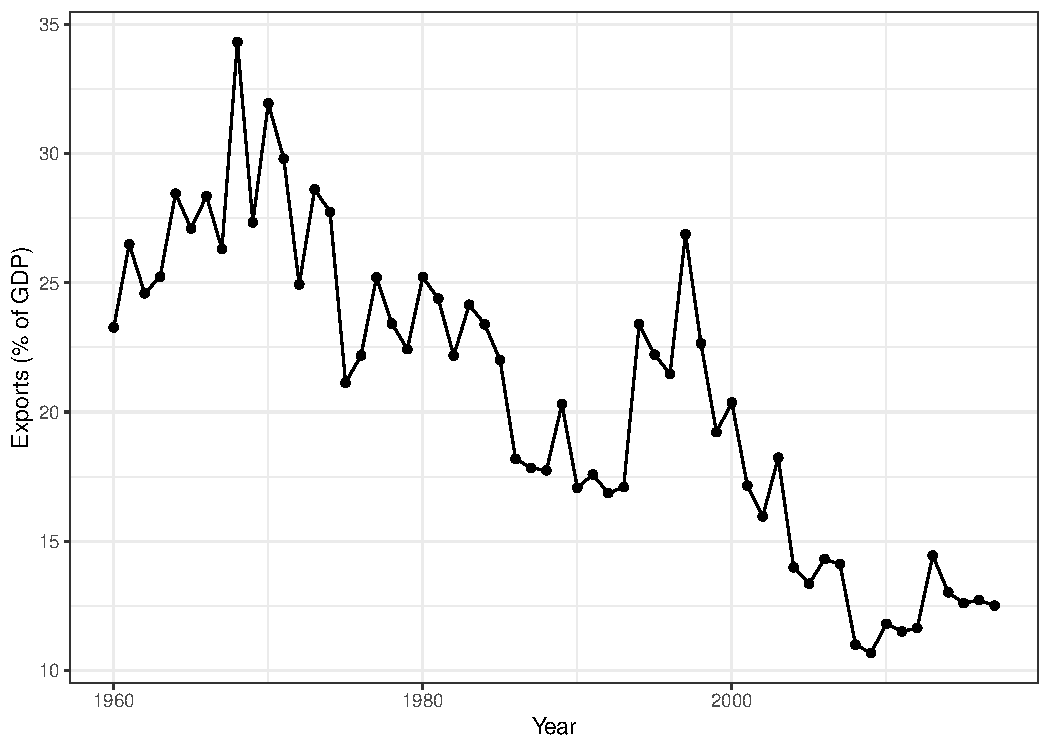
\includegraphics[width=0.675\textwidth]{fig/car-1.pdf}
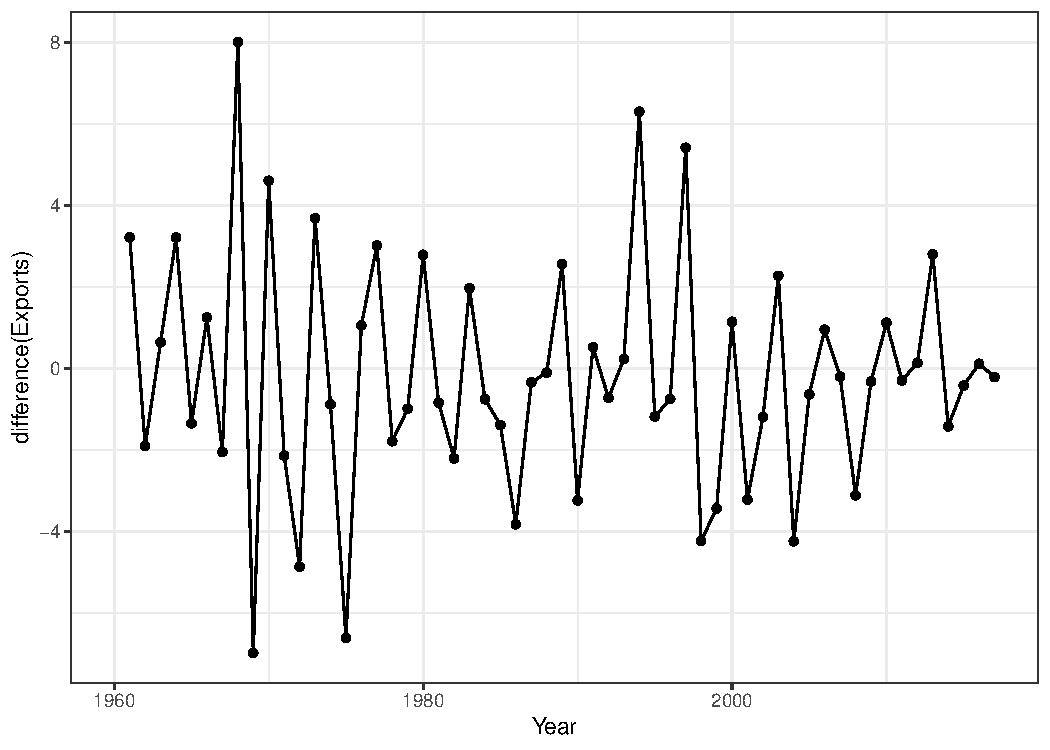
\includegraphics[width=0.675\textwidth]{fig/car-2.pdf}
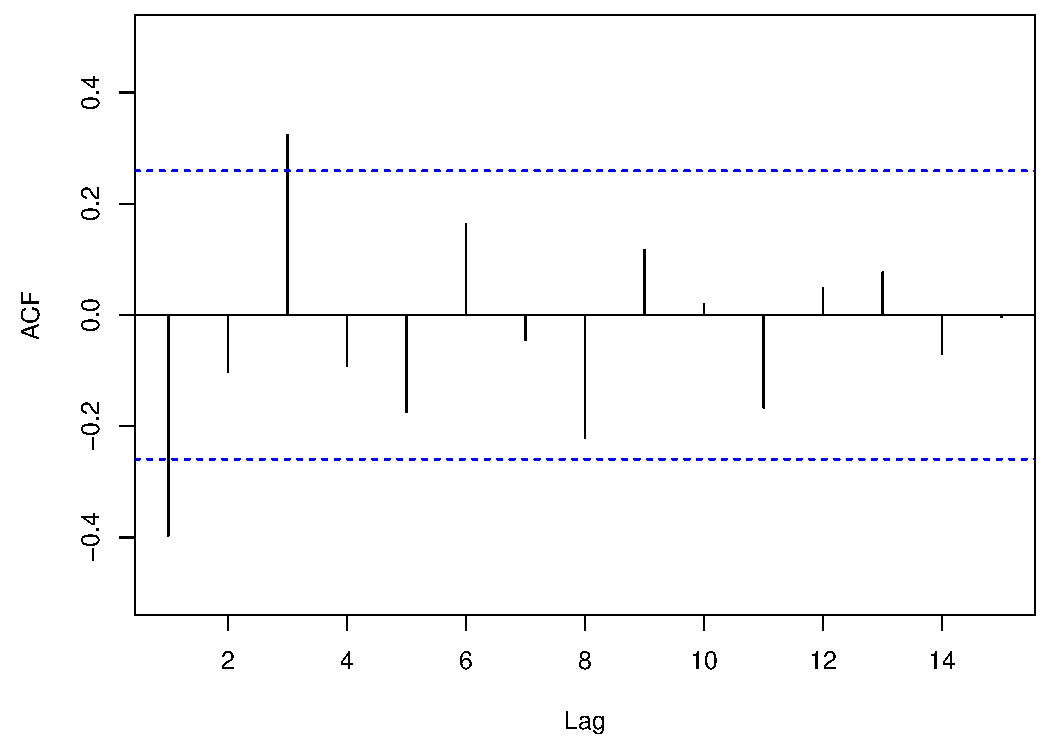
\includegraphics[width=0.45\textwidth]{fig/car-3.pdf}
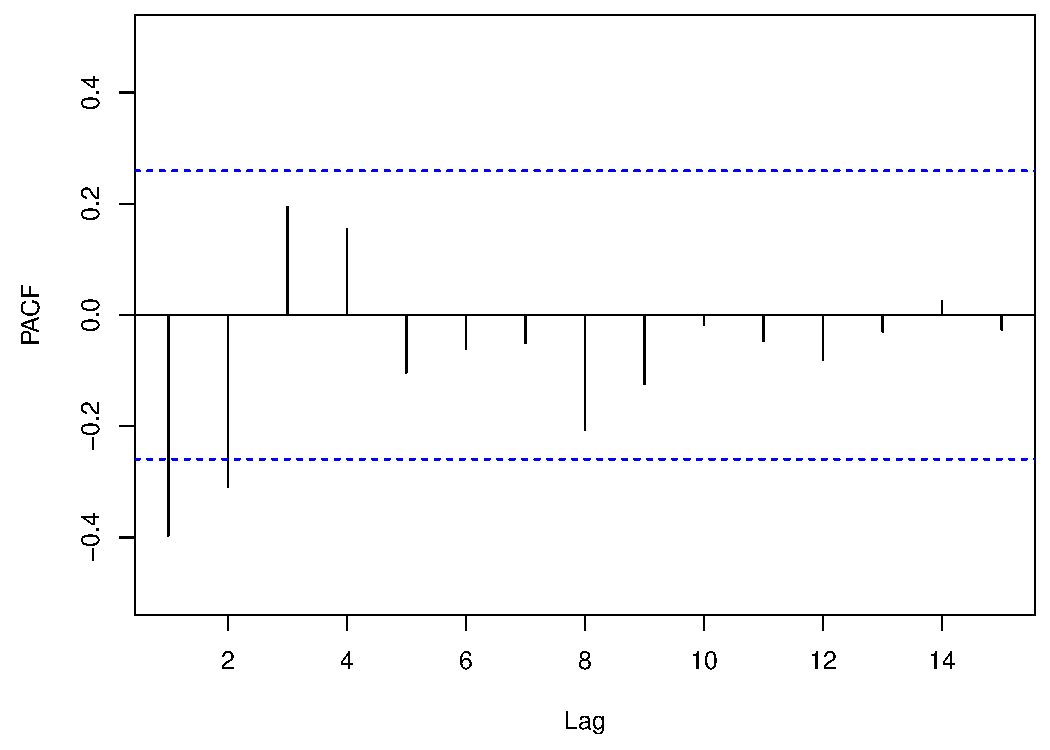
\includegraphics[width=0.45\textwidth]{fig/car-4.pdf}
\caption{Top row: exports (as a percentage of GDP) for Central African
  Republic (from HA). Middle row: first differences of exports. Bottom row: ACF 
  and PACF functions of first differences.}
\label{fig:car_exploratory}
\end{figure}

\item ACF and PACF plots are shown in the third row of Figure
  \ref{fig:car_exploratory}. To be clear, these are applied to first differences
  of the data. They are suggestive of MA(3) and AR(2) dynamics,
  respectively. Thus we can go and fit each model: ARIMA(2,1,0) and ARIMA(0,1,3)
  (note that these are ARIMA models with $d=1$, since we are going to specify
  the differencing as part of the model itself). We can also use the
  Hyndman-Khandakar algorithm. This ends up choosing ARIMA(2,1,2)   

\item For prediction-focused tasks (and probably/necessarily, longer sequences),
  we would look at an estimate of (say) MAE using time series cross-validation
  to help us choose a model. Here, HA recommend looking at AICc, which is what
  is also built into the \verb|fable| package's reporting of the \verb|ARIMA()| 
  output. This leads us to choose ARIMA(2,1,0). The residuals from this model
  also look close to white noise (see the R notebook for diagnostics) which is
  good  

\item Forecasts from our fitted ARIMA(2,1,2) model are shown in the rop row of
  Figure \ref{fig:car_forecast}, for a 5-year horizon. Also plotted are
  prediction intervals around the forecast (more on this in the last 
  section). Qualitatively, the forecasts aren't very impressive at first
  glance---they look more or less like what we'd get if we used a random walk
  (zero mean function, growing variance function), which is just ARIMA(0,1,0)   

\begin{figure}[p]
\centering
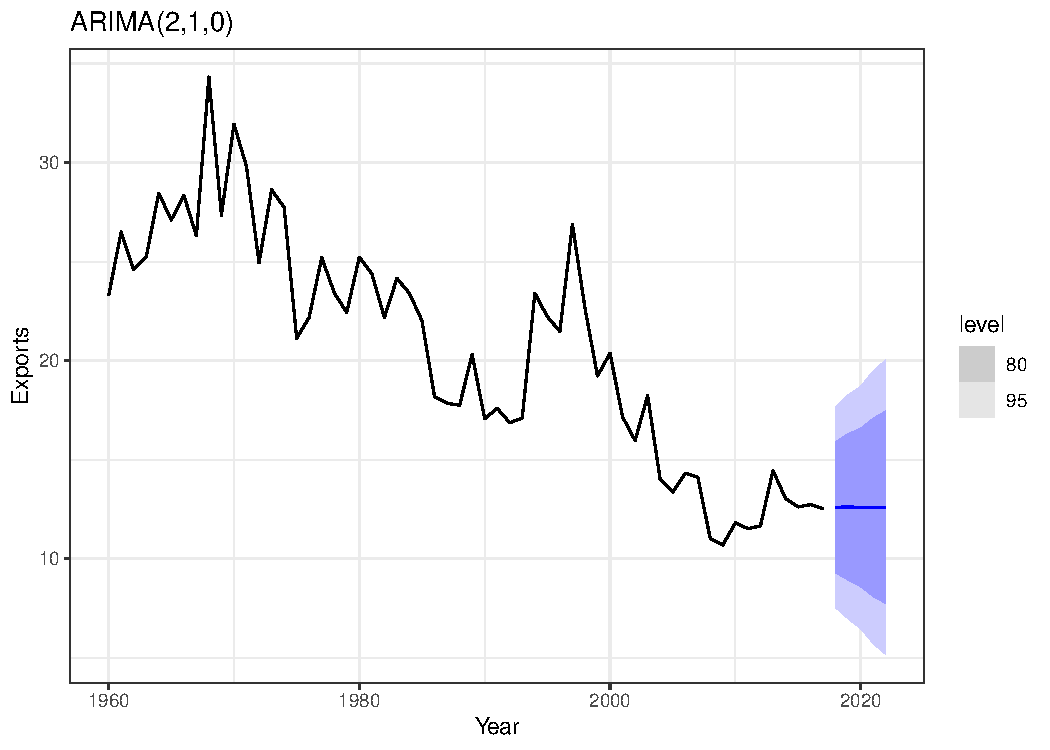
\includegraphics[width=0.825\textwidth]{fig/car-7.pdf}
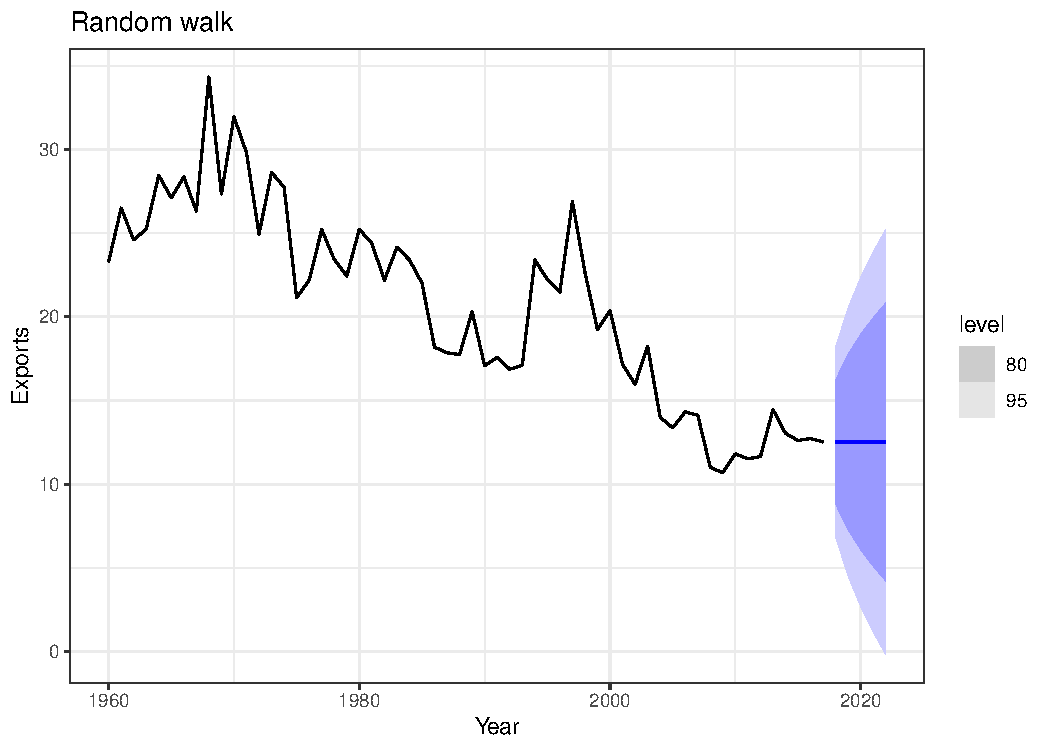
\includegraphics[width=0.825\textwidth]{fig/car-8.pdf}
\caption{Top row: forecasts from ARIMA(2,1,2). Bottom row: forecasts from
  ARIMA(0,1,0) with $c=0$, i.e., a random walk.}
\label{fig:car_forecast}
\end{figure}

\item However, HA comment that the prediction intervals here are narrower than
  they would be for a random walk, which is due to the contribution of the
  nontrivial AR and MA components that we've been able to pick up and model. To
  check this, we plot forecasts from ARIMA(0,1,0) in the bottom row of Figure
  \ref{fig:car_forecast}, and indeed you can see they have wider uncertainty 
  bands 

\item A general note to close out our example: the \verb|ARIMA()| function in
  the \verb|fable| package can be handy \emph{but also a bit dangerous} because
  it may automate away some part of the model building procedure even when you 
  think you've specified a model manually. Check out the R notebook for an
  example and guidance on how to explicitly get what you want ... 
\end{itemize}

\subsection{Seasonality extensions}

\begin{itemize}
\item Seasonality is typically handled in ARIMA models by seasonal
  differencing. This assumes that the seasonal periods are known

\item For example, let's suppose that the seasonal period is known to be
  $s$. Then, to start off as simple as possible, a \emph{purely seasonal ARMA}
  model with orders $P,Q \geq 0$ and period $s$, denoted ARMA$(P,Q)_s$, is of 
  the form   
  \begin{equation}
  \label{eq:pure_sarma_pq}
  \Phi(B^s) x_t = \Theta(B^s) w_t  
  \end{equation}
  where $\Phi(B^s) = 1 - \Phi_1 B^s - \Phi_2 B^{2s} - \cdots - \Phi_P B^{Ps}$
  and $\Theta(B) = 1 + \Theta_1 B + \Theta_2 B^{2s} + \cdots + \Theta_Q
  B^{Qs}$. Note that these model AR and MA dynamics, but on the scale of
  seasons: since all backshifts are in multiples of $s$

\item To select orders for seasonal dynamics we would follow ideas just like
  those for regular (nonseasonal) ARMA models: look at ACF and PACF plots,
  \emph{but for lags on the seasonal scale}, in multiples of $s$ 

\item To make this more sophisticated, we can add in AR and MA dynamics on
  the original scale, which leads to a \emph{seasonal ARMA} model of orders 
  $p,q,P,Q \geq 0$ and period $s$, denoted ARMA$(p,q)(P,Q)_s$,   
  \begin{equation}
  \label{eq:sarma_pq}
  \phi(B) \Phi(B^s) x_t = \theta(B) \Theta(B^s) w_t  
  \end{equation}
  where $\phi(B) = 1 - \phi_1 B - \phi_2 B^2 - \cdots - \phi_p B^p$ and
  $\theta(B) = 1 + \theta_1 B + \theta_2 B^2 + \cdots + \theta_q B^q$ are the AR 
  and MA operators, as before, and $\Phi(B^s), \Theta(B^s)$ are the seasonal
  operators, as above

\item The full scale sophistication is achieved by adding in integration to
  account for nonstationarity. However, now we can also account for
  nonstationarity on the seasonal scale; first define a $D\th$ order seasonal
  difference eperator
  \[
  \nabla_s^D = (1 - B^s)^D 
  \]
  Then define the \emph{seasonal ARIMA} (SARIMA) model of orders $p,d,q,P,D,Q 
  \geq 0$ and period $s$, denoted ARIMA$(p,d,q)(P,D,Q)_s$, 
  \begin{equation}
  \label{eq:sarima_pdq}
  \phi(B) \Phi(B^s) \nabla^d \nabla_s^D x_t = \theta(B) \Theta(B^s) w_t  
  \end{equation}
  As usual, we are omitting an intercept $c$ for simplicity, but in general we
  could include this on the right-hand side in \eqref{eq:sarima_pdq}. (Phew!
  That's the full beast. We've maxed out in complexity, at least for this
  lecture ...) 

\item Estimation is even more complicated in SARIMA models (more parameters, 
  more nonlinearity) but thankfully software does it for us

\item We won't go into any further details than what we have discussed already,
  but will walk through an example from HA to model (and forecast) US
  employment numbers in leisure/hospitality. The data is shown in Figure
  \ref{fig:leisure_exploratory}, top row. It has a clear seasonal pattern with
  (safe guess) a 1 year period  

\item Taking seasonal differences (i.e., applying $\nabla_s$ with $s = 12$,
  since this is monthly data) has removed the seasonality, but the result, in
  the middle row of Figure \ref{fig:leisure_exploratory}, is still very clearly
  nonstationary   

\item Additionally taking monthly differences (i.e., applying the composite 
  operator $\nabla \nabla_s$), in the bottom row of Figure
  \ref{fig:leisure_exploratory}, is reasonably stationary-looking    

\begin{figure}[p]
\centering
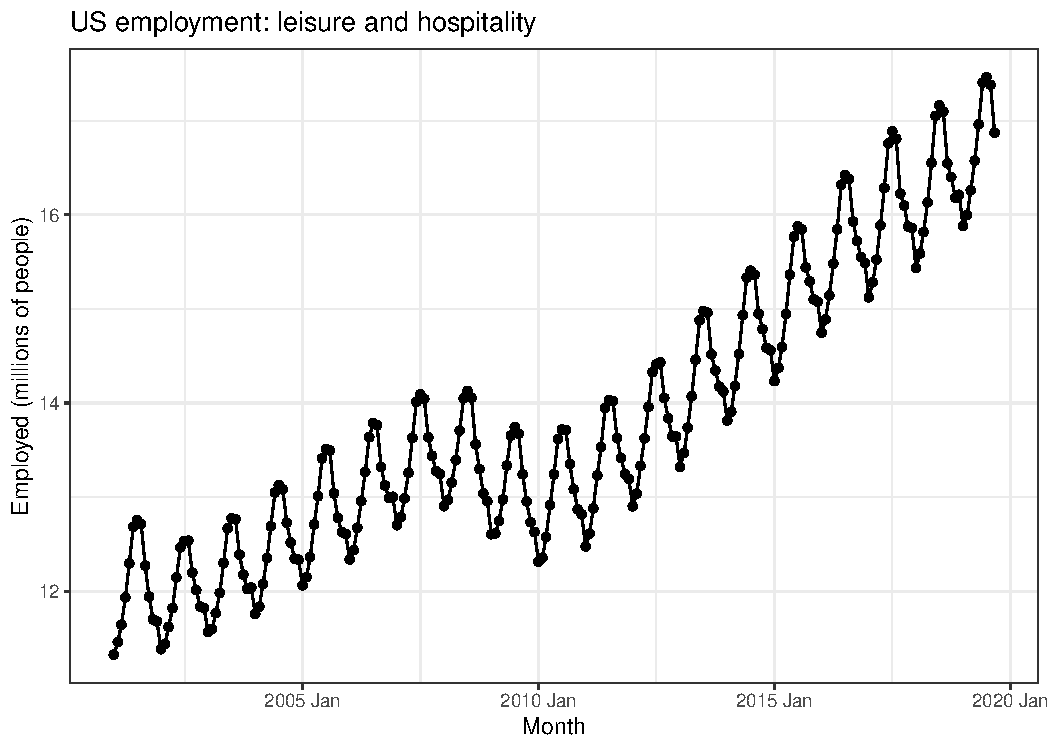
\includegraphics[width=0.6\textwidth]{fig/leisure-1.pdf}
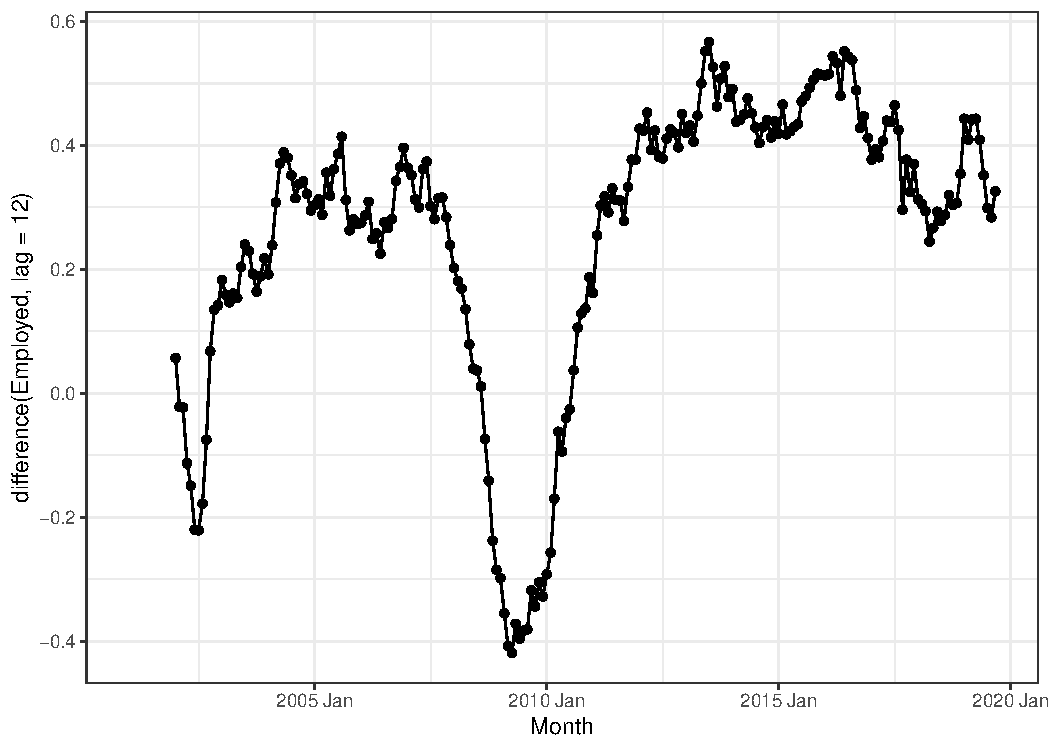
\includegraphics[width=0.6\textwidth]{fig/leisure-2.pdf}
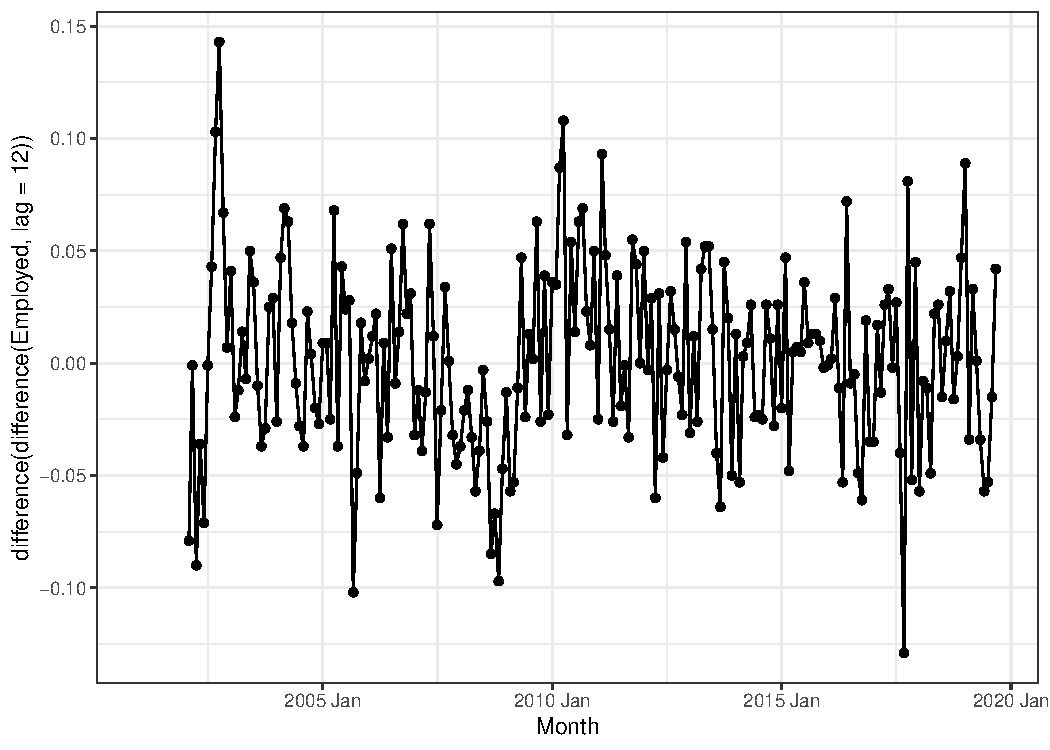
\includegraphics[width=0.6\textwidth]{fig/leisure-3.pdf}
\caption{Top row: number of US jobs (in millions) in leisure/hospitality (from
  HA). Middle row: seasonal (yearly) differences. Bottom row: differences of
  seasonal differences.} 
\label{fig:leisure_exploratory}
\end{figure}

\item ACF and PACF plots are displayed in the top row of Figure
  \ref{fig:leisure_forecast}. To be clear, these are applied to the differences
  of yearly differences ($\nabla \nabla_s x_t$, $t = 1,2,3,\dots$, as plotted in
  the bottom row of Figure \ref{fig:leisure_forecast}). The ACF shows two
  moderate correlations at lags 1 and 2 and then a big spike at lag 12. This is
  suggestive of an nonseasonal MA(2) and a seasonal MA(1), and thus we can go
  and fit an ARIMA$(0,1,2)(0,1,1)_{12}$ model. Meanwhile, the PACF shows again
  to moderate correlations at lags 1 and 2 and a big spike at lag 12. This
  suggests a nonseasonal AR(2) and a seasonal AR(1), so we can go and fit an
  ARIMA$(2,1,0)(1,1,0)_{12}$ model. Lastly, we can also try the
  Hyndman-Khandakar algorithm. This ends up choosing ARIMA$(1,1,1)(2,1,1)_{12}$  

\begin{figure}[htb]
\centering
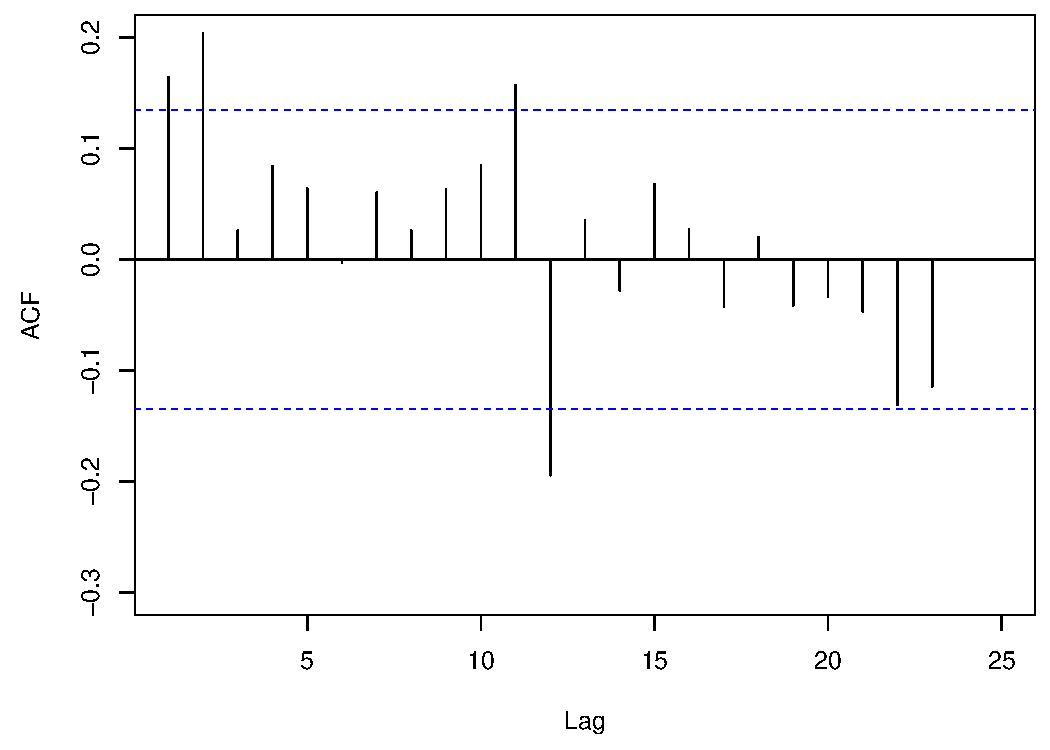
\includegraphics[width=0.45\textwidth]{fig/leisure-4.pdf}
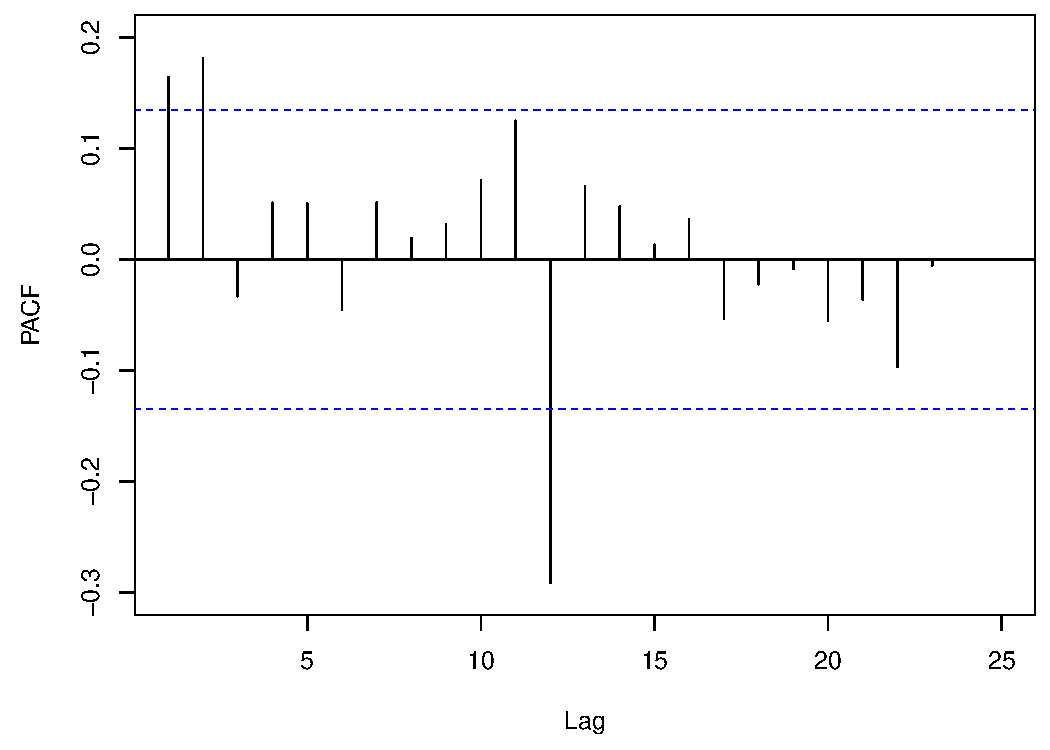
\includegraphics[width=0.45\textwidth]{fig/leisure-5.pdf}
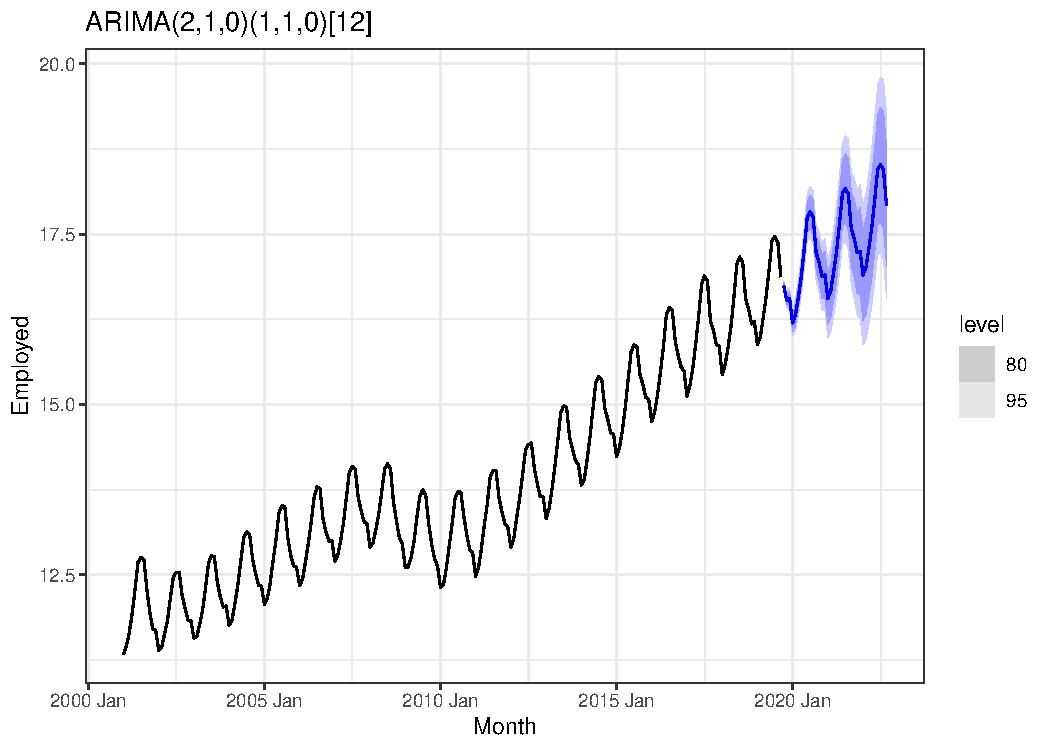
\includegraphics[width=0.825\textwidth]{fig/leisure-8.pdf}
\caption{Top row: ACF and PACF functions of differences of seasonal
  differences. Bottom row: forecasts from ARIMA(2,1,2).}
\label{fig:leisure_forecast}
\end{figure} 

\item AICc (see the R notebook for details and diagnostics)
  tells us to choose the ARIMA$(1,1,1)(2,1,1)_{12}$ model. But that seems a bit 
  doubtful because it suggests there is a second-order autoregressive dynamic 
  on the yearly scale, which makes the model much more complicated. As usual,
  if we cared about prediction, then we should probably just use time series
  cross-validation to evaluate the different models. More on this in the
  forecasting section. For now, we'll just produce 3-year forecasts from the 
  ARIMA$(0,1,2)(0,1,1)_{12}$ model

\item These are shown in the bottom row of \ref{fig:leisure_forecast}. They
  actually seem fairly plausible and interesting. Note that the seasonality was
  nicely captured by the seasonal differencing, and the increasing trend seems
  to have been nicely captured by the nonseasonal differencing
\end{itemize}

\section{Forecasting}

\begin{itemize}
\item ARIMA models, especially with seasonality extensions, can be powerful 
  forecasters, as we've seen in a couple of examples. Some authors treat
  torecasting with ARIMA in a complex and notation-heavy way, but in fact it can
  be explained intuitively (which we borrow from HA)

\item As before, we will use the notation \smash{$\hat{x}_{t+h | t}$} to denote
  a forecast of $x_{t+h}$ made using data up through $t$

\item Some potentially helpful nomenclature: $t+h$ here is called the
  \emph{target time} (time of the target we are trying to forecasting), and $t$
  is called the \emph{forecast time} (time at which we make the forecast) 

\item Obtaining the forecast \smash{$\hat{x}_{t+h | t}$} from an ARIMA model can 
  be done by iterating the following steps: 

\begin{enumerate}
\item Start with the ARIMA equation
  \[
  \phi(B) \Phi(B^s) \nabla^d \nabla_s^D x_t = c + \theta(B) \Theta(B^s) w_t   
  \]
  Plug in for parameter estimates, and rearrange so that $x_t$ is on the
  left-hand side an all other terms are on the right-hand side 

\item Rewrite the equation by replacing $t$ with $t+h$

\item On the right-hand side of the equation, replace future observations
  ($x_{t+k}$, $k \geq 1$) with their forecasts, future errors ($w_{t+k}$, $k
  \geq 1$) with zero, and past errors ($w_{t-k}$, $k \geq 0$) with their ARIMA 
  residuals   
\end{enumerate}

\item Beginning with $h = 1$, we iterate this procedure for $h = 2,3,\dots$ as
  needed to get the forecasts at the ultimate horizon we desire  

\item It helps to walk through an example. Consider forecasting with a fitted 
  ARIMA(3,1,1) model, which we start by writing as
  \[
  (1 - \hat\phi_1 B - \hat\phi_2 B^2 - \hat\phi_3 B^2) (x_t - x_{t-1}) = \hat{c}
  + (1 + \hat\theta_1 B) w_t
  \]

\item We expand this as 
  \[
  x_t - \hat\phi_1 x_{t-1} - \hat\phi_2 x_{t-2} - \hat\phi_3 x_{t-3} - 
  (x_{t-1} - \hat\phi_1 x_{t-2} - \hat\phi_2 x_{t-3} - \hat\phi_3 x_{t-4}) = 
  \hat{c} + w_t + \hat\theta_1 w_{t-1}
  \]

\item And rearrange as
  \[
  x_t = \hat{c} + (1 + \hat\phi_1) x_{t-1} + (\hat\phi_2 - \hat\phi_1) x_{t-2} + 
  (\hat\phi_3 - \hat\phi_2) x_{t-3} - \hat\phi_3 x_{t-4} + w_t + \hat\theta_1
  w_{t-1} 
  \]

\item To make a 1-step ahead forecast, we first replace $t$ by $t+1$ above:  
  \[
  x_{t+1} = \hat{c} + (1 + \hat\phi_1) x_t + (\hat\phi_2 - \hat\phi_1) x_{t-1} + 
  (\hat\phi_3 - \hat\phi_2) x_{t-2} - \hat\phi_3 x_{t-3} + w_{t+1} +
  \hat\theta_1 w_t  
  \]
  and then we set $w_{t+1} = 0$, and replace $w_t$ by \smash{$\hat{w}_t$}, which
  is the residual from our fitted ARIMA model, yielding 
  \[
  \hat{x}_{t+1 | t} = \hat{c} + (1 + \hat\phi_1) x_t + (\hat\phi_2 - \hat\phi_1)
  x_{t-1} + (\hat\phi_3 - \hat\phi_2) x_{t-2} - \hat\phi_3 x_{t-3} +
  \hat\theta_1 \hat{w}_t  
  \]

\item To make a 2-step ahead forecast, we similarly start with 
  \[
  x_{t+2} = \hat{c} + (1 + \hat\phi_1) x_{t+1} + (\hat\phi_2 - \hat\phi_1) x_t +
  (\hat\phi_3 - \hat\phi_2) x_{t-1} - \hat\phi_3 x_{t-2} + w_{t+2} +
  \hat\theta_1 w_{t+1}
  \]
  and then we set $w_{t+2} = w_{t+1} = 0$, and replace $x_{t+1}$ by
  \smash{$\hat{x}_{t+1 | t}$}, yielding  
  \[
  \hat{x}_{t+2 | t} = \hat{c} + (1 + \hat\phi_1) \hat{x}_{t+1 | t} + (\hat\phi_2
  - \hat\phi_1) x_t + (\hat\phi_3 - \hat\phi_2) x_{t-1} - \hat\phi_3 x_{t-2}  
  \]

\item This process can be iterated any number of times to obtain forecasts
  arbitrarily far into the future 
\end{itemize}

\subsection{Behavior of long-term forecasts}

\begin{itemize}
\item \emph{Should} we keep iterating the process above to generate forecasts
  arbitrarily far into the future? 

\item The answer is almost certainly ``no'', in most applications! You should 
  be more careful. Short of detecting and projecting seasonality, ARIMA models
  are limited for long-term forecasts (in general, long-term forecasts are very
  hard without precise domain-specific knowledge of what the long-range dynamics
  look like ... and even then, many domains to not offer much to say there ...)  

\item It is important to have a qualitative sense of what long-term forecasts
  look like in ARIMA. Again, we borrow this nice explanation from HA. Starting
  with \eqref{eq:arima_pdq_c}, a nonseasonal ARIMA model, we can break down the
  explanation into cases (recall $c$ is the intercept, and $d$ is the
  differencing order):  

\begin{enumerate}
\item If $c = 0$ and $d = 0$, then the long-term forecasts will converge
  to zero 
\item If $c = 0$ and $d = 1$, then the long-term forecasts will converge
  to a nonzero constant 
\item If $c = 0$ and $d = 2$, then the long-term forecasts will follow a
  linear trend
\item  If $c \not= 0$ and $d = 0$, then the long-term forecasts will
  converge to the historical mean 
\item  If $c \not= 0$ and $d = 1$, then the long-term forecasts will
  follow a linear trend
\item  If $c \not= 0$ and $d = 2$, then the long-term forecasts will
  follow a quadratic trend (can be dangerous! some software packages do not
  allow $d \geq 2$ when $c \not= 0$ ...)
\end{enumerate}

\item You will verify this on your homework for some simple ARIMA models, where
  you'll also work out the qualitative behavior for long-term forecasts from
  seasonal ARIMA models 
\end{itemize}

\subsection{Split-sample and cross-validation}

\def\SplitMSE{\mathrm{SplitMSE}} 
\def\CVMSE{\mathrm{CVMSE}}

\begin{itemize}
\item At last, we arrive to our bread-and-butter tools for evaluating ARIMA  
  models for their predictive accuracy: split-sample and time series
  cross-validation (CV) 

\item They apply exactly as described in the regression lecture: to recap, in
  split-sample validation, we pick a time $t_0$, train our model (regression,
  ARIMA, whatever) on data up through $t_0$, and then we evaluate forecasts  
  \smash{$\hat{x}_{t |  t_0}$} over times $t > t_0$:
  \[
  \SplitMSE = \frac{1}{n-t_0} \sum_{t = t_0+1}^n \big( \hat{x}_{t | t_0} - x_t
  \big)^2   
  \]
  In time series CV, we use data before $t_0$ as a burn-in period (usually we
  would choose a smaller $t_0$ here than for split-sample) to ensure the initial
  model is decent, and then iteratively retrain at each $t > t_0$ in order to
  make forecasts. For $h$-step ahead forecasts:    
  \[
  \CVMSE = \frac{1}{n-t_0} \sum_{t = t_0+1}^n \big( \hat{x}_{t | t-h} - x_t
  \big)^2    
  \]
  (Instead of MSE, we could also use MAE, or MAPE, or MASE as our metric ...) 

\item There is not much more to say other than to reiterate that these are our
  most robust (assumption-lean) tools for assessing utility in a predictive 
  context. You'll get continued practice with time series CV on your
  homework. The \verb|fable| package that we'll use for a lot of forecasting
  tools has a handy (though memory-inefficient) way of implementing this, which
  saves you from writing a loop by hand 

\item There is one important warning to give however! This applies to
  cross-validation, generally, in any setting. Cross-validation evaluates the
  prediction error of \emph{an entire procedure}. Thus the entire procedure
  \emph{must be rerun} each time predictions are to be validated. So, e.g., if
  we are using auto-ARIMA (as implemented by \verb|ARIMA()| in the \verb|fable|
  package) to select an ARIMA order for us, then we must rerun auto-ARIMA at
  each time $t > t_0$ in order to evaluate forecasts in the last display. (And,
  note, it will generally pick different orders at each $t > t_0$ ... the way to
  think about it is that we are evaluating the prediction error of auto-ARIMA 
  \emph{procedure} itself, not any particular selected order) 

\item In other words, we \emph{cannot} run auto-ARIMA once over all time, and
  then take the selected ARIMA order and apply this retrospectively. That would
  not yield an honest estimate of prediction error (since we would have used the 
  future at $t > t_0$ to select the ARIMA order). Summary:

\begin{center}
\begin{tabular}{|l|l|}
\hline
Wrong way: & 
\parbox[c]{0.77\textwidth}{ \smallskip
Run auto-ARIMA at time $n$ (all time) to select $p,d,q$, and use this 
retrospectively in time series CV to fit ARIMA($p,d,q$) at each $t > t_0$ and
make forecasts \smallskip}  
\\ \hline
Right way: & 
\parbox[c]{0.77\textwidth}{ \smallskip
Run auto-ARIMA at each $t > t_0$ to select (time-dependent) $p,d,q$, and use
this to fit ARIMA($p,d,q$) and make forecasts in time series CV \smallskip} 
\\ \hline
\end{tabular}  
\end{center}

\item (Note: we are not advertising or advocating for the use of auto-ARIMA, but
  are simply explaining that this would be the right way to validate it) 

\item Finally, as a rule-of-thumb, we recall Occam's razor: if a number of
  models all have reasonably similar split-sample or cross-validated prediction
  error, then we would generally prefer to use the simplest among them 
\end{itemize}

\subsection{Prediction intervals}

\begin{itemize}
\item The predictions \smash{$\hat{x}_{t+h | t}$} from ARIMA described above are 
    known as \emph{point forecasts}. But if you look back at Figures
    \ref{fig:car_forecast} and \ref{fig:leisure_forecast}, you can see bands
    around the point forecasts (which are the dark lines) 

\item These bands represent \emph{prediction intervals}, which are typically
  quite important in practice, since they reflect uncertainty in the predictions 
  that are made (and can be useful for downstream decision-making)  

\item There are various ways to compute prediction intervals. One method is to
  obtain an estimate \smash{$\hat\sigma^2_h$} of the variance of the ``$h$-step
  ahead forecast distribution''. This is in quotes because we have not defined
  this precisely, and we will avoid going into details because this approach is
  not always tractable, and also requires more assumptions about the ARIMA
  model, including (typically) normality of the noise distribution. But in any
  case, having computed such an estimate, we could model the $h$-step ahead
  forecast distribution at time $t$ as
  \[
  N\big( \hat{x}_{t+h | t}, \hat\sigma^2_h \big)
  \]
  and compute prediction intervals accordingly. For example, to compute a
  central 90\% prediction interval, we would use 
  \[
  \big[\hat{x}_{t+h | t} - \hat\sigma_h q_{0.95}, \, \hat{x}_{t+h | t} +  
  \hat\sigma_h q_{0.95} \big]
  \]
  where $q_{0.95}$ is the 0.95 quantile of the standard normal distritbuion

\item Another method is adapt the method described previously to iteratively
  produce point forecasts to instead iteratively produces samples paths from the
  forecast distribution. This is what is done in the \verb|fable| package's
  \verb|forecast()| function when \verb|bootstrap = TRUE|. The gist of the idea
  is as follows: in step 3, instead of replacing future errors ($w_{t+k}$, $k
  \geq 0$) by zero, we replace them by a bootstrap draw (i.e., a uniform sample
  with replacement) from the empirical distribution of past residuals. Given a
  bunch of sample paths, we can then read off empirical quantiles at $t+h$ for a
  prediction interval  

\item Unfortunately, neither of these methods (nor any other traditional
  methods) for producing prediction intervals are guaranteed to actually give
  \emph{coverage} in practice. That is, you would hope that our 95\% prediction 
  intervals actually cover 95\% of the time, but this need not be the case

\item Fortunately, we will learn that there are some relatively simple
  correction methods that can act as post-processors to endow any given sequence
  of prediction intervals with long-run coverage. We will talk about this near the 
  end of the course when we discuss calibration  
\end{itemize}

\subsection{ARIMAX models}

\begin{itemize}
\item In practice, including auxiliary features in an ARIMA model can make it
  much more powerful. This is true in general: finding good predictors can make
  a huge difference in forecasting!

\item Auxiliary features are often referred to as \emph{exogenous} in the
  context of time series models, and an ARIMA model with exogenous predictors is
  often abbreviated ARIMAX 

\item Formally, an ARIMAX($p,d,q$) model is an extension of the ARIMA model 
  \eqref{eq:arima_pdq} of the form 
  \[
  \phi(B) \nabla^d x_t = \beta^\T u_t + \theta(B) w_t
  \]
  where $u_t$, $t = 0, \pm 1, \pm 2, \pm 3, \dots$ is an exogenous predictor
  sequence 

\item Forecasting with ARIMAX models is a little more complicated because, for
  ``true'' ex-ante forecasts, we will typically not have the values of the
  exogenous predictor available that we need (think about the steps we outlined
  for forecasting with ARIMA models, and how we substituted future observations
  with their forecasted values---unless we build a separate forecast model for
  $u_t$, we will not know how to impute them) 

\item As usual (as we described in the regression lecture), we can use lagged
  exogenous features as predictors in order to circumvent this issue

\item (Note: be careful not to confuse an ARIMAX model with a regression with 
  correlated errors! They are not the same thing. In both models, there are
  exogenous predictors and and errors with MA dynamics, but the distinguishing  
  factor is the AR dynamic: in an ARIMAX model, the ``response'', which is $x_t$
  in our notation here, exhibits AR dynamics; in a regression with correlated
  errors, the errors exhibit AR dynamics) 
\end{itemize}

\subsection{IMA models}

\begin{itemize}
\item Forecasting with the ARIMA(0,1,1) model, also written as IMA(1,1), bears
  an interesting connection to what is called \emph{simple exponential 
    smooting} (SES). This is also sometimes called an \emph{exponentially
    weighted moving averages} (EWMA) forecaster. It tends to be popular in
  economics (SS call it ``frequently used and abused'')     

\item To develop the connection, consider the IMA model with an MA coefficient
  of $\theta = -(1-\alpha)$, where $0 < \alpha < 1$. We can write this as  
  \[
  x_t - x_{t-1} = w_t - (1-\alpha) w_{t-1}
  \]

\item Because $\alpha < 1$, this has an invertible representation: writing $y_t
  = x_t - x_{t-1}$, recall what we developed in \eqref{eq:ma_1_invertible},
  which yields 
  \[
  w_t = \sum_{j=0}^\infty (1-\alpha)^j y_{t-j} 
  \]
  or
  \[
  y_t = -\sum_{j=1}^\infty (1-\alpha)^j y_{t-j} + w_t
  \]
  
\item Substituting $y_t = x_t - x_{t-1}$, and rearranging, this gives 
  \begin{align*}
  x_t &= x_{t-1} - \sum_{j=1}^\infty (1-\alpha)^j (x_{t-j} - x_{t-j-1}) + w_t \\
  &= x_{t-1} + \sum_{j=1}^\infty (1-\alpha)^j x_{t-j-1} - \sum_{j=1}^\infty
    (1-\alpha)^j x_{t-j} + w_t \\
  &= \sum_{j=1}^\infty (1-\alpha)^{j-1} x_{t-j} - \sum_{j=1}^\infty (1-\alpha)^j
    x_{t-j} + w_t \\
  &= \sum_{j=1}^\infty \alpha (1-\alpha)^{j-1} x_{t-j} + w_t 
  \end{align*}

\item The 1-step ahead prediction from this model is therefore  
  \begin{align*}
  \hat{x}_{t+1 | t} &= \sum_{j=1}^\infty \alpha (1-\alpha)^{j-1} x_{t+1-j} \\  
  &= \alpha x_t + \sum_{j=2}^\infty \alpha (1-\alpha)^{j-1} x_{t+1-j} 
    \\
  &= \alpha x_t + \sum_{j=1}^\infty \alpha (1-\alpha)^j x_{t-j} \\
  &= \alpha x_t + (1-\alpha) \sum_{j=1}^\infty \alpha (1-\alpha)^{j-1}
    x_{t-j} \\
  &= \alpha x_t + (1-\alpha) \hat{x}_{t | t-1}
  \end{align*}

\item In other words, the 1-step ahead prediction is a weighted combination of
  the current observation $x_t$ and the previous prediction \smash{$\hat{x}_{t |
      t-1}$}

\item Smaller values of $\alpha$ (closer to 0) lead to smoother forecasts, since
  we are ``borrowing'' more from the previous forecast, in the last
  display

\item This is the simplest in a class of methods based on exponential smoothing,
  which we will cover in the next lecture
\end{itemize}
\end{document}
